\documentclass[11pt,twoside]{report}


% some definitions for the title page
\newcommand{\reporttitle}{A New Scalable Runtime for LLM Inference}
\newcommand{\reportauthor}{Hamish McCreanor}
\newcommand{\supervisor}{Peter Pietzuch}
\newcommand{\reporttype}{MEng Individual Project}
\newcommand{\degreetype}{MEng Computing} 

% load some definitions and default packages
%%%%%%%%%%%%%%%%%%%%%%%%%%%%%%%%%%%%%%%%%
% University Assignment Title Page 
% LaTeX Template
% Version 1.0 (27/12/12)
%
% This template has been downloaded from:
% http://www.LaTeXTemplates.com
%
% Original author:
% WikiBooks (http://en.wikibooks.org/wiki/LaTeX/Title_Creation)
%
% License:
% CC BY-NC-SA 3.0 (http://creativecommons.org/licenses/by-nc-sa/3.0/)
% 
%
%%%%%%%%%%%%%%%%%%%%%%%%%%%%%%%%%%%%%%%%%
%----------------------------------------------------------------------------------------
%	PACKAGES AND OTHER DOCUMENT CONFIGURATIONS
%----------------------------------------------------------------------------------------
\usepackage[a4paper,hmargin=2.8cm,vmargin=2.0cm,includeheadfoot]{geometry}
\usepackage{textpos}
\usepackage{natbib} % for bibliography
\usepackage{tabularx,longtable,multirow,subfigure,caption}%hangcaption
\usepackage{fncylab} %formatting of labels
\usepackage{fancyhdr} % page layout
\usepackage{url} % URLs
\usepackage[english]{babel}
\usepackage{amsmath}
\usepackage{graphicx}
\usepackage{dsfont}
\usepackage{epstopdf} % automatically replace .eps with .pdf in graphics
\usepackage{backref} % needed for citations
\usepackage{array}
\usepackage{latexsym}
\usepackage[pdftex,pagebackref,hypertexnames=false,colorlinks]{hyperref} % provide links in pdf
\usepackage{verbatim}

\hypersetup{pdftitle={},
  pdfsubject={}, 
  pdfauthor={},
  pdfkeywords={}, 
  pdfstartview=FitH,
  pdfpagemode={UseOutlines},% None, FullScreen, UseOutlines
  bookmarksnumbered=true, bookmarksopen=true, colorlinks,
    citecolor=black,%
    filecolor=black,%
    linkcolor=black,%
    urlcolor=black}

\usepackage[all]{hypcap}


%\usepackage{color}
%\usepackage[tight,ugly]{units}
%\usepackage{float}
%\usepackage{tcolorbox}
%\usepackage[colorinlistoftodos]{todonotes}
% \usepackage{ntheorem}
% \theoremstyle{break}
% \newtheorem{lemma}{Lemma}
% \newtheorem{theorem}{Theorem}
% \newtheorem{remark}{Remark}
% \newtheorem{definition}{Definition}
% \newtheorem{proof}{Proof}


%%% Default fonts
\renewcommand*{\rmdefault}{bch}
\renewcommand*{\ttdefault}{cmtt}



%%% Default settings (page layout)
\setlength{\parindent}{0em}  % indentation of paragraph

\setlength{\parindent}{0em}  % indentation of paragraph

\setlength{\headheight}{14.5pt}
\pagestyle{fancy}
\renewcommand{\chaptermark}[1]{\markboth{\chaptername\ \thechapter.\ #1}{}} 
%\fancyhead[RO]{\sffamily \textbf{\thepage}} %Page no.in the right on even pages
%\fancyhead[LE]{\sffamily \textbf{\thepage}} %Page no. in the left on odd pages

\fancyfoot[ER,OL]{\thepage}%Page no. in the left on
                                %odd pages and on right on even pages
\fancyfoot[OC,EC]{\sffamily }
\renewcommand{\headrulewidth}{0.1pt}
\renewcommand{\footrulewidth}{0.1pt}
\captionsetup{margin=10pt,font=small,labelfont=bf}


%--- chapter heading

\def\@makechapterhead#1{%
  \vspace*{10\p@}%
  {\parindent \z@ \raggedright \sffamily
    \interlinepenalty\@M
    \Huge\bfseries \thechapter \space\space #1\par\nobreak
    \vskip 30\p@
  }}

%--- chapter heading

\def\@makechapterhead#1{%
  \vspace*{10\p@}%
  {\parindent \z@ \raggedright \sffamily
        %{\Large \MakeUppercase{\@chapapp} \space \thechapter}
        %\\
        %\hrulefill
        %\par\nobreak
        %\vskip 10\p@
    \interlinepenalty\@M
    \Huge\bfseries \thechapter \space\space #1\par\nobreak
    \vskip 30\p@
  }}

%---chapter heading for \chapter*  
\def\@makeschapterhead#1{%
  \vspace*{10\p@}%
  {\parindent \z@ \raggedright
    \sffamily
    \interlinepenalty\@M
    \Huge \bfseries  #1\par\nobreak
    \vskip 30\p@
  }}	
\allowdisplaybreaks


% load some macros
% Here, you can define your own macros. Some examples are given below.

\newcommand{\R}[0]{\mathds{R}} % real numbers
\newcommand{\Z}[0]{\mathds{Z}} % integers
\newcommand{\N}[0]{\mathds{N}} % natural numbers
\newcommand{\C}[0]{\mathds{C}} % complex numbers
\renewcommand{\vec}[1]{{\boldsymbol{{#1}}}} % vector
\newcommand{\mat}[1]{{\boldsymbol{{#1}}}} % matrix


% load title page
\begin{document}
% Last modification: 2015-08-17 (Marc Deisenroth)
\begin{titlepage}

\newcommand{\HRule}{\rule{\linewidth}{0.5mm}} % Defines a new command for the horizontal lines, change thickness here

%----------------------------------------------------------------------------------------
%	LOGO SECTION
%----------------------------------------------------------------------------------------


\includegraphics[width = 4cm]{./figures/imperial}\\[0.5cm] 

\center % Center everything on the page
 
%----------------------------------------------------------------------------------------
%	HEADING SECTIONS
%----------------------------------------------------------------------------------------

\textsc{\LARGE \reporttype}\\[1.5cm] 
\textsc{\Large Department of Computing}\\[0.5cm] 
\textsc{\large Imperial College of Science, Technology and Medicine}\\[0.5cm] 

%----------------------------------------------------------------------------------------
%	TITLE SECTION
%----------------------------------------------------------------------------------------

\HRule \\[0.4cm]
{ \huge \bfseries \reporttitle}\\ % Title of your document
\HRule \\[1.5cm]
 
%----------------------------------------------------------------------------------------
%	AUTHOR SECTION
%----------------------------------------------------------------------------------------

\begin{minipage}{0.4\textwidth}
\begin{flushleft} \large
\emph{Author:}\\
\reportauthor % Your name
\end{flushleft}
\end{minipage}
~
\begin{minipage}{0.4\textwidth}
\begin{flushright} \large
\emph{Supervisor:} \\
\supervisor % Supervisor's Name
\end{flushright}
\end{minipage}\\[4cm]




%----------------------------------------------------------------------------------------


%----------------------------------------------------------------------------------------
%	DATE SECTION
%----------------------------------------------------------------------------------------

{\large \today} % Date, change the \today to a set date if you want to be precise


\vfill % Fill the rest of the page with whitespace
Submitted in partial fulfillment of the requirements for the \degreetype~of Imperial College London

\end{titlepage}



% page numbering etc.
\pagenumbering{roman}
\clearpage{\pagestyle{empty}\cleardoublepage}
\setcounter{page}{1}
\pagestyle{fancy}

%%%%%%%%%%%%%%%%%%%%%%%%%%%%%%%%%%%%
\begin{abstract}

\begin{comment}
Test-time compute scaling has emerged as a recent alternative to expensive training processes for improving LLM performance.
Approaches in this paradigm produce chains of reasoning steps in response to a user query, often sampling multiple outputs at a time in order to explore a search space of possible answers.
In this paper we consider beam search, a test-time compute scaling method that makes use of one model to generate reasoning steps (the LLM) and another model (the PRM) to score these steps and guide a tree search towards a response.
Such collaborative LLM workflows are relatively unsupported and there exist substantial opportunities to optimise the performance profile of these multi-model systems.
In particular, we explore the memory characteristics of a beam search system implemented in the popular vLLM library, seeking to analyse the memory requirements of both models, their individual optimal batching strategies as well as how overall system performance changes as the memory split between the two models varies.
We also conduct experiments to evaluate the effectiveness of vLLM's KV cache management strategy, finding it optimal for a tree-search usage pattern.
\end{comment}

Test-time compute scaling has emerged as an alternative to expensive training for improving large language model (LLM) performance. 
Methods in this paradigm generate chains of reasoning in response to a user query, often sampling multiple outputs to explore a space of possible answers. 
This paper focuses on beam search, a test-time compute scaling approach that uses one model (the LLM) to generate reasoning steps and another (the process-reward model, or PRM) to score and guide a tree search toward a final response.

Such collaborative systems are relatively underexplored, and significant opportunities remain to optimise their performance.
We examine the memory characteristics of a beam search system implemented using the popular vLLM inference library, analysing the memory usage and batching behaviour of both models, and how system performance varies with different memory allocations between them.
Additionally, we evaluate vLLM’s KV cache management strategy and find it well-suited to tree-search-style workloads. 

Building on these insights, we propose a decoupled tree exploration strategy that exploits differing batching preferences between the LLM and PRM to improve system throughput.
We use the results of our investigations to quantify the potential benefits of such an optimisation.

\end{abstract}

\cleardoublepage
%%%%%%%%%%%%%%%%%%%%%%%%%%%%%%%%%%%%
\section*{Acknowledgments}
I would like to thank my supervisor, Professor Peter Pietzuch, for his invaluable guidance throughout this project.
I am also deeply grateful to members of Imperial College London's Large-Scale Data and Systems Group, in particular Marcel Wagenländer, whose support and insights were instrumental to this work.

Finally, I wish to thank my flatmates, Adam Maltby, Cameron Fraser, and Om Singh, as well as my parents, Peter and Annie McCreanor, for their unwavering support and encouragement throughout the project.
%\clearpage{\pagestyle{empty}\cleardoublepage}

%%%%%%%%%%%%%%%%%%%%%%%%%%%%%%%%%%%%
%- table of contents
\fancyhead[RE,LO]{\sffamily {Table of Contents}}
\tableofcontents 


%\clearpage{\pagestyle{empty}\cleardoublepage}
\pagenumbering{arabic}
\setcounter{page}{1}
\fancyhead[LE,RO]{\slshape \rightmark}
\fancyhead[LO,RE]{\slshape \leftmark}

%%%%%%%%%%%%%%%%%%%%%%%%%%%%%%%%%%%%
\chapter{Introduction} % 1-3 pages
% What is the problem?
% Why is it interesting?
% How do I propose to solve it?
\begin{comment}
  
\end{comment}

As large language models (LLMs) are adopted for an ever-growing range of applications, scaling time spent in training has emerged as the dominant paradigm for improving model performance.
However, with training costs growing prohibitively expensive, there is increasing interest in other techniques for bettering model output. 
Test-time compute scaling offers one such way to improve performance, with existing models achieving better results by ``thinking'' for longer.
This is done by encouraging LLMs to output longer chains of reasoning, shifting scaling costs from training time to test time and enabling existing models to improve without incurring any extra training expense.

The most popular test-time compute scaling approaches leverage a second model to guide a tree-search towards the best answer.
A generator LLM proposes steps to an answer to a user query and a verifier LLM scores these steps, with this process repeating until a set criteria is met. 
This is a departure from an assumption made by existing LLM inference systems, which is that only one model will run at a time.
As such, they are likely to have made architectural decisions that limit the throughput and latency of a test-time scaling approach involving the interplay between multiple LLMs.

This represents an opportunity to build a new system that more effectively supports the test-time scaling use case.
Key to these efforts is optimizing the memory of such a system, particularly the management of the key-value (KV) cache, which stores intermediate results reused during autoregressive token generation. 
Efficient use of the KV cache can significantly improve memory utilisation and computational speed.

This project analyses a beam search implementation built upon vLLM, a popular and widely used LLM inference library, to try and identify deficiencies that limit the effective use of GPU memory. 
Several experiments are conducted to better understand how the implementation's performance changes as a function of various parameters and optimisations to improve GPU memory utilisation are proposed and validated. 

%%%% Add bit here explaining what optimisations I tried

%%%
%%%%%%%%%%%%%%%%%%%%%%%%%%%%%%%%%%%%
\chapter{Background} % 10-20 pages
We provide an overview of transformer architecture in \ref{section:llmarchitecture}, as well as key components of the inference pipeline in \ref{section:llminference}, before detailing the idea of test-time compute scaling and describing relevant techniques in \ref{section:testtimecompute}.
\section{LLM Architecture}\label{section:llmarchitecture}
\subsection{Transformer Architecture}
While the term ``Large Language Model'' can be used to describe any model trained on large volumes of textual data, it is frequently used to refer to models that use a variant of the transformer architecture described in \cite{vaswani2017attention}.
This architecture has superseded recurrent neural networks for language-based tasks owing to its ability to capture long range dependencies between tokens.
It does this via a unique attention mechanism.
This, and the other components present in a transformer, are described below.
\begin{itemize}
  \item \textbf{Embedding Layers:} 
    Attention blocks are fed a matrix where each row represents the semantic meaning of each token. This is done by using an embedding learnt during the training process and applying this to the input tokens.
  \item \textbf{Positional Encoding:} 
    Unlike recurrent neural networks, transformer models contain no a priori knowledge of the order of the input sequence.
    To remedy this, positional encodings are added to the input embeddings before they are fed to the attention block.
    There are several ways of doing this, however the approach adopted in the \cite{vaswani2017attention} is to use apply sine and cosine functions to the position and dimension of the input vector as follows:
    \begin{equation*}
      \begin{split}
        \textnormal{PE}_{(pos, 2i)} = sin(pos/10000^{2i/d_{model}}) \\ 
        \textnormal{PE}_{(pos, 2i+1)} = cos(pos/10000^{2i/d_{model}})
      \end{split}
    \end{equation*}
  \item \textbf{Multi-Head Attention:}
    Transformers use an attention block to describe the relationship between different tokens in a sequence. 
    This takes as input a key, query and value matrix $K$, $Q$, $V$ respectively. 
    The key and query matrices are multiplied together to produce a representation of how each token in the sequence relates to each other token.
    After normalising and applying a softmax function, the matrix is multiplied by $V$, which represents the semantic meaning of each input token.
    \begin{equation*}
      \textnormal{Attention}(Q,K,V) = \textnormal{softmax}(\frac{QK^T}{\sqrt{d_k}})V
    \end{equation*}
    In practise, multiple attention heads are used and their outputs concatenated.  
    Instead of attention blocks just operating on the $K$, $Q$, and $V$ directly, they are multiplied by learned matrices $W^K$, $W^Q$, and $W^V$ to project the input vectors into different spaces.
    The fact that there are multiple of these matrices $W_i^Q$, $W_i^K$ and $W_i^V$ allows the model to attend to information learnt from different projections concurrently.
    \begin{equation*}
      \begin{split}
        \textnormal{MultiHead}(Q,K,V) = \textnormal{Concat}(\textnormal{head}_1, ..., \textnormal{head}_h)W^O \\
        \textnormal{where} \: \textnormal{head}_i = \textnormal{Attention}(QW_i^Q, KW^K_i, VW^V_i)
      \end{split}
    \end{equation*}
  \item \textbf{Position-wise Fead-Forward Networks:} 
    The output of the multi-head attention block is fed to a fully connected neural-network.
    This takes as input the representation at each position (making it ``position-wise'') and applies two linear transformations separated by a ReLU activation:
    \begin{equation*}
      \textnormal{FFN}(x) = \textnormal{max}(0, xW_1 + b_1)W_2 + b_2
    \end{equation*}
\end{itemize}
Multiple blocks consisting of the multi-head attention and feed-forward layers are stacked on top of one another to produce a deeper transformer model.
\subsubsection{Model Variants}
The encoder-decoder model introduced in \cite{vaswani2017attention} is not the only variant of the transformer architecture that exists.
Modifications to the transformer architecture have been made in order to better support different tasks:  
\begin{itemize}
  \item \textbf{Encoder-decoder:}
    With encoder-decoder models, an input sequence is first embedded, then added to a positional encoding before being passed as input to a stack of attention and feed-forward network layers (the ``encoder'') to produce a representation of the input sequence. 
    As the output sequence is generated, it is fed as input to a similarly structured ``decoder'' block. 
    This takes an embedded output sequence, with positional encoding, as input.
    The output of the encoder block is fed to attention blocks in the decoder block in order to model the relationship between the input and output sequence.
    These models \cite{raffel2020exploring} tend to be used for tasks like sequence to sequence transformation, for example language translation.
  \item \textbf{Encoder-only:}
    Encoder-only models use only the encoder block of an encoder-decoder model to produce a vector representation of an input sequence.
    These models do not produce text directly, but are instead meant to pass their output to a downstream component for further inference, potentially for applications to sentiment analysis or named-entity recognition.
    Examples of these include the BERT \cite{kenton2019bert} family of models.
  \item \textbf{Decoder-only:}
    Decoder-only models like those in the GPT \cite{radford2018improving} series make up the bulk of models used for auto-regressive text generation and completion. 
    Instead of sending an input prompt to an encoder block, the prompt is instead passed in in conjuction to the output sequence and the model is trained to predict the next token in the sequence \cite{dai2015semi}.
\end{itemize}

\section{LLM Inference}\label{section:llminference}
We begin with an overview of the steps taken to perform inference for a single request, before detailing other important aspects of LLM inference like managing the KV cache, distributing computation across multiple compute nodes and request batching.
\subsection{Inference Pipeline}\label{subsection:inferencepipeline}
Performing inference based on a user prompt involves a prefill phase to initialise the state of the transformer model followed by an autoregressive phase to generate an output sequence.
These steps are sandwiched by tokenisation and detokenisation stages respectively in order to convert between a string and vector representation of the input and output sequence.
\begin{itemize}
  \item \textbf{Tokenisation:}
    In order to convert from a string representation of an input sequence, to a vector representation that a model can understand, tokenisation is applied.
    This splits the input string into a sequence of tokens present in a vocabulary learnt from the training corpus \cite{radford2019language} \cite{sennrich2015neural}, producing a vector of indices for each token in the input string.
    These indices are used to index into the learnt embeddings matrix and extract an embedding vector for each input token.
  \item \textbf{Prefill phase:}
    The prefill phase refers to the stage in the inference pipeline at which the hidden states (keys and values) of the network from the input sequence are produced.
    These values are later used to generate output tokens.
    Additionally, KV cache entries (see \ref{subsection:kvcache}) for these tokens are produced and are later used to speed up the autoregressive phase of the inference pipeline.
    This stage represents an operation over a large matrix and, as such, can saturate the GPU, making this stage largely arithmetic bound.
  \item \textbf{Autoregressive phase:}
    In the autoregressive phase (also referred to as the decode phase), output tokens are generated incrementally and appended back to the output prompt. 
    The final layer of the transformer produces a probability distribution over all output tokens (typically using a softmax activation), which is sampled from to produce an output token.
    A temperature parameter can be introduced to modify this probability distribution and control the level of randomness present in the sampling stage.
    Since we are only generating one token at a time, this phase is typically bound by the rate at which vectors can be passed to GPU memory.
    Further, the sequential dependencies between outputs limits the parallelisability of the autoregressive phase.
    The sequential nature of the autoregressive phase, and its corresponding performance characteristics, has significantly shaped the design of existing LLM runtimes (see \ref{chapter:relatedwork}).
  \item \textbf{Detokenisation:}
    At the end of the autoregressive phase, a vector containing indices into the model vocabulary is produced - this represents the output sequence of the model.
    In order to convert this vector to a string representation, the vector is sent to the CPU and each element is used to index into the model vocabulary, producing a string for each token.
    This list of token strings is then joined to form the overall output string.
\end{itemize}

\subsection{KV Cache}\label{subsection:kvcache}
The KV cache represents an important area with which inference efficiency can be improved.
During the autoregressive phase of inference, self-attention refers to the key and value vectors $KW_i^K$ and $VW_i^V$ as well as the query vector of the latest output token.
These key and value vectors have already been calculated at prior iterations and so caching them can reduce the computational overhead at each autoregressive step, as we can use these vectors without recalculation.
The computed key and value vectors for the newest token are then added to the KV cache, to be reused during the next autoregressive iteration.
This cache is initially populated during the prefill phase but then grows with the output sequence length. 
The effective management of the KV cache can be used to help overcome the limited parallelisability of the autoregressive phase of inference \cite{shi2024keep} \cite{pope2023efficiently}.

\subsection{Hardware}
The recent success of LLMs is in large part enabled by the use of Graphics Processing Units (GPUs) \cite{krizhevsky2012imagenet}.
GPUs are optimised for performing a large number of specialised operations in parallel, in contrast with Central Processing Units (CPUs), which are better suited to performing a more general set of operations sequentially.
Modern deep neural networks can be distilled down into a sequence of vector and matrix operations.
These tasks are highly parallelisable and specialised implementations like of linear algebra operations like cuBLAS \cite{cublas} exist to accelerate them on GPU hardware.
Other software layers like CUDA \cite{nickolls2008scalable} also exist and can be used to implement efficient versions of common deep learning functions.  
As a result of this, GPUs are well suited for the kind of workloads required by LLMs. 

At a high level, GPUs consist of a series of Streaming Multiprocessors (SMs), each containing multiple Stream Processors (SPs, also referred to as `cores') and some shared memory\cite{choquette2021nvidia}. 
Each core is designed to support a small set of relatively simple operations, like floating-point and integer arithmetic, as well as logical operations.
High-bandwidth memory (HBM) is used to transfer data between SMs, while the shared memory on each SM can be used to share common data between threads.
Tensors like weights and the KV cache are typically stored in HBM and then moved into the SMs at the time of computation \cite{pope2023efficiently}.

% explore other hardware platforms - asics, fpgas, tpus
In addition to GPUs, other hardware platforms like ASICs, FPGAs and TPUs exist and can be used to further accelerate the operations of LLMs \cite{li2024large}.
These platforms tend to be more heterogenous in architecture and, as such, most existing LLM runtimes (see \ref{chapter:relatedwork}) tend to be optimised for a GPU-like architecture.

\subsection{Distributed Computation}
One approach to scaling LLMs to is to distribute computation amongst multiple GPUs. 
Model data can be shared across multiple nodes in a network to increase inference throughput, while model layers and even individual tensors can be sharded to enable the deployment of larger models.
These techniques need not be used in isolation and are frequently used in combination in existing training and inference pipelines \cite{kwon2023efficient} \cite{shoeybi2019megatron} \cite{yu2022orca}.
\begin{itemize}
  \item \textbf{Data parallelism:} Data parallelism involves replicating the weights for an entire model across multiple nodes.
    Each node is now capable of handling inference requests independently, increasing the number of requests that can be serviced in parallel.  
    This approach reduces request latency and is simple to implement and scale, but has high memory requirements, as each node must be capable of storing the weights for the entire model as well as any intermediate tensors produced during inference.
    This is potentially prohibitive for larger models featuring high numbers of weights \cite{rae2021scaling} \cite{brown2020language} \cite{chowdhery2023palm} .
  \item \textbf{Pipeline parallelism:} Pipeline parallelism is a way to distribute computation that enables training and inference for models with a large number of weights.
    This approach borrows from the classic computer architecture technique of pipelining \cite{hennessy2011computer}.
    Nodes are assigned the weight tensors for individual layers of the network and are responsible for executing that layer alone.
    Data is then passed between nodes in sequence \cite{huang2019gpipe}.
    This method incurs a small computational overhead in moving data between nodes in the pipeline, however this is relatively minor compared to the scheduling delay incurred in other methods like tensor parallelism.
    The main drawback of this method is the potential for bubbles to form in the pipeline.
    This occurs due to nodes taking different times to compute their layer.
    Nodes that complete early might have to wait idle while nodes upstream of them in the pipeline execute, reducing node utilisation.
  \item \textbf{Tensor parallelism:} Tensor parallelism extends pipeline parallelism to allow the deployment of models whose layers or intermediate tensors may be too large to fit on just one node.
    Layer specific tensors, like weights or intermediate activations can be sharded across multiple nodes. 
    Nodes then work together to complete a subset of the overall tensor computation before combining their results later.
    While this approach enables even larger models to be executed, it further increases the computational overhead of sharing data across nodes - we now need to synchronise and move data on an intra-layer basis, instead of on an inter-layer basis as in pipeline parallelism \cite{shoeybi2019megatron}.
\end{itemize}

\subsection{Request Batching}
Another method used to address the limited parallelism created by the autoregressive phase of inference is to batch requests. 
With request batching, we can stack tensors from multiple user requests into the same batch and issue this request to the GPU.
This enables user requests to be served in parallel and increases GPU utilisation at the same time as maximising use of available memory bandwith.

\begin{itemize}
  \item \textbf{Naive batching:} The naive approach to batching consists of grouping multiple input prompts into a batch and running inference on it - inference is scheduled at the granularity of requests \cite{yu2022orca}.
    In order for the input and output batches to be valid matrix shapes, they must be padded with special padding tokens to a fixed size.
    While simple to implement, this approach can lead to increased latency as well as underutilisation of the GPU. 
    This is because prompts within a batch do not necessarily generate output sequences of the same length. 
    If one output sequence has terminated while there are other sequences for which tokens are still being generated it will be unable to be returned to the user until all other sequences terminate.
    As such the request latency is bounded by the time taken to generate the longest sequence in the batch \cite{yu2022orca}.
    This also limits the system from serving new requests as they arrive: the new request will need to wait for completion of the entire batch of requests, even if the batch contains requests for which an output has already been generated.
    As a result, naive batching is limited in its use, only achieving maximal GPU utilisation under very specific usage patterns.

  \item \textbf{Continuous batching:} Continuous batching is proposed as an improvement to naive batching and schedules inference at the granularity of autoregressive iterations \cite{yu2022orca}.
    At the end of each autoregressive iteration, a set of new tokens is produced for every request in the batch.    
    A scheduler then monitors the batch to determine the completion status of every request in the batch, dynamically scheduling waiting requests when it detects that a complete output sequence has been generated.
    This achieves greater utilisation of the GPU since it is no longer executing operations for sequences that have already terminated.
    It also reduces latency for user requests, as output sequences can be returned as soon as they are terminated.
    However, this batching technique comes at the cost of increased scheduling overhead as well as limited batching of certain matrix operations.
    This is because some operations, like computing attention, require their input sequences to be aligned to the same length and position in order to be batched.
    Because requests are dynamically dispatched, this property no longer holds and thus operations like computing attention blocks are unabled to be batched, in a technique known as ``selective batching'' \cite{yu2022orca}.
\end{itemize}

\section{Test Time Compute Scaling}\label{section:testtimecompute}
Historically, approaches to improving LLM performance have centered on training. 
With larger datasets, larger models and more training epochs, performance on the cross-entropy loss function used for training these models can be made to improve considerably \cite{kaplan2020scaling}.  
However, scaling in this way eventually becomes prohibitively expensive due to the high cost of owning and operating the hardware required for training.

This motivates the idea of test-time compute scaling.
Test-time compute scaling trades off inference latency for higher quality responses to user prompts. 
By allowing existing LLMs to take longer to respond to user prompts, the quality of responses can be improved considerably \cite{snell2024scaling}, obviating the need to retrain a bigger model on a more expansive dataset.
Test-time compute scaling describes a broad approach to trading off inference latency for higher quality model outputs - specific methodologies for how to implement this are described below.

\subsection{Chain of Thought Prompting}
Chain of thought prompting uses a series of reasoning steps to improve LLM answer quality.  
By prompting a model with examples of answers containing structured reasoning steps and encouraging it to follow a similar structure in its own responses, model performance has been empirically shown to improve considerably \cite{wei2022chain}.

\subsection{Self Consistency Sampling}
Self-consistency sampling is a simple technique to improve model outputs that replaces the decoding strategy present in chain of thought prompting.
Instead of greedily sampling each token, self-consistency voting generates a diverse set of reasoning paths by sampling multiple tokens in parallel.
These tokens produce a tree structure, with different branches corresponding to different token choices.
When all reasoning paths conclude with an answer to the user's question, the answers from all paths are aggregated out by majority vote to produce a final response \cite{wang2022self}.

\subsection{Best-of-N Sampling}
Best-of-N sampling extends the idea of self-consistency to include some sort of external verifier.
This verifier can be any machine learning model but is typically some sort of transformer model.
In the basic best-of-n setup, this verifier scores all the n solutions sampled from the LLM and the one with the highest score is output as the final response.
With weighted best-of-n, all the final solutions are aggregated such that reasoning paths that generate the same solution are weighted higher when combined with the verifier score \cite{stiennon2020learning}.  

\subsection{Beam Search}
Beam search provides a way of systematically exploring the tree structure created when generating multiple chains of reasoning in parallel. 
Multiple chains of reasoning are generated iteratively, with scores being output for each step.
These scores are then used to guide the search towards higher quality answers - reasoning steps with higher scores are expanded through further sampling and reasoning steps with lower scores are pruned \cite{feng2023alphazero} \cite{yao2023tree}. 

We maintain a fixed number $N$ of active paths and expand each of these paths with $M$ samples. 
All of these $N \times M$ new reasoning steps are scored and the top $N$ steps are kept for the next iteration. 

Implementations of beam search frequently use a Process Reward Model (PRM) to score the intermediate reasoning steps. 
PRMs differ from the verifier models used in best-of-n search in that they are trained to output a score for every reasoning step, rather than just the final result.

%% Include a diagram of some sort

\chapter{Related Work}\label{chapter:relatedwork}
% speak about different runtimes and their contributions
Various runtimes for performing LLM inference already exist.
These implement some of the techniques described earlier in order to provide efficient inference for a variety of use cases.
In order to understand where it might be possible to offer a novel contribution with regard to performance, we first need to understand the features offered by existing solutions.
Here we present a selection of popular runtimes and detail their main contributions and points of difference.
\section{Inference Runtimes}\label{section:inferenceruntimes}
\subsection{vLLM}
vLLM is a popular LLM runtime designed for high throughput serving of inference requests \cite{kwon2023efficient}.
It addresses key challenges in memory management that arise during LLM serving, particularly those related to KV cache memory.
Existing systems often suffer from memory inefficiencies due to fragmentation and over-allocation, limiting their ability to process large batch sizes effectively.
vLLM solves this problem through a novel memory management mechanism called PagedAttention, achieving near-zero KV cache waste \cite{kwon2023efficient}.
The rest of the vLLM system is built to support this use of PagedAttention and integrates several other common optimisation techniques, including continuous batching, as well as pipeline and tensor parallelism.
It supports a variety of popular LLMs, including those in the GPT, OPT and LLaMA series \cite{radford2018improving} \cite{zhang2022opt} \cite{touvron2023llama}.

\subsubsection{PagedAttention}
The main contribution of vLLM is its PagedAttention mechanism. 
On receiving a new request, many inference runtimes pre-allocate a contiguous chunk of memory for the KV cache equal in size to the request's maximum output.
This can cause internal fragmentation, if the actual output is less than the size of memory allocated, as well as external fragmentation, when smaller requests are unable to be scheduled due to overallocation.
Moreover, for requests that generate multiple outputs, as is the case with parallel and beam search, the KV cache is stored in a different location for each output and so there is no possibility of memory reuse.

To address this, PagedAttention divides the request's KV cache into smaller units called blocks. 
These contain a fixed number of key and value vectors associated with a set of tokens. 
Blocks for a given request's KV cache need not be located in physically contiguous locations and are allocated dynamically as the KV cache for a request grows. 
This eliminates external fragmentation as each block is the same size.
The blocks themselves are chosen to be small in size in order to limit internal fragmentation \cite{kwon2023efficient}.
This is analagous to the paging technique common to modern operating systems \cite{kilburn1962one}, with blocks corresponding to pages, tokens to bytes and requests to processes \cite{kwon2023efficient}.

By passing only the necessary KV cache blocks to the GPU kernel for each request, vLLM avoids overallocation and enables tighter packing of data from multiple requests into a single kernel invocation. 
This effectively increases the batch size and leads to significantly improved throughput.

\subsubsection{Automatic Prefix Caching}\label{subsubsection:automatic_prefix_caching}
The KV cache blocks used by PagedAttention provide a natural mechanism through which prefix caching can be implemented.
Prefix caching is a technique common to many inference runtimes to avoid recomputing KV cache values across shared input prompts.
The KV cache blocks of processed requests are cached and reused when a new request comes in with a shared prefix.


To handle this automatic prefix caching, vLLM introduces a KV cache manager.
It maintains a doubly linked list of free KV cache blocks, as well as a list of currently cached KV blocks in use.
When a new request arrives, vLLM computes hash values for the token sequences in the request - these hashes are derived not only from the current tokens but also from the sequence of prefix tokens that precedes them. 
If a matching hash is found, indicating that the KV cache blocks for those tokens have already been computed, they can be directly reused by the new request.
In the event of a prefix cache miss, vLLM allocates new KV cache blocks by popping from the list of free blocks and populating them with the computed KV values for the unmatched prefix.
If no free KV cache blocks are available, vLLM evicts blocks from the cache. 
Eviction is done based on a least-recently-used (LRU) policy, with a preference for evicting the blocks associated with the longest prefixes first, as these are less likely to be shared by future requests.
% diagram


\subsubsection{Architecture}
vLLM exposes a Python library and an OpenAI API \cite{openaiapi} compatible web server for inference.
The frontend is written using the FastAPI library \cite{fastapi}.
Python is used to implement the bulk of the project, with C++ and CUDA code being used to implement the custom CUDA kernels required to support the PagedAttention mechanism.
Importantly, control-specific components like the batch scheduler are implemented in Python, representing a potential source of overhead.

vLLM uses a heirarchical class structure to distribute requests amongst GPU workers.
A single executor is maintained through the lifespan of the runtime.
This is responsible for creating and running worker processes.
These are processes dedicated to running model inference on specific GPUs and are tasked with preparing tensors and orchestrating the execution of the model on that node. 
Importantly, this means that a separate Python process needs to be created for every single worker node, incurring a performance penalty.

On individual GPU workers, a block engine is used to allocate a contiguous chunk of GPU RAM and divide it into physical KV cache blocks.
A block manager is created to maintain the mapping between logical and physical KV blocks and this is also implemented in Python. 
NCCL \cite{nccl} is used for communication across distributed GPU workers.

\subsection{SGLang}
SGLang is an inference runtime designed to efficiently execute LLM-centric programs that involve multiple, often dependent, generation calls interleaved with control flow and structured inputs/outputs \cite{zheng2024sglang}. 
Unlike traditional inference engines focused solely on throughput or latency, SGLang provides a frontend programming interface and a backend runtime to optimise execution for multi-call, structured LLM workflows.

At the frontend, SGLang provides a domain-specific language embedded in Python. 
It exposes that allow users to express parallelism, control flow, and constrained generation.
This enables modular, composable, and readable construction of LLM workflows.

The backend runtime, known as SGLang Runtime (SRT), introduces three main contributions: 
\begin{itemize}
  \item \textbf{RadixAttention:} A mechanism for automatic KV cache reuse across multiple generation calls, using a radix tree to manage shared prompt prefixes. 
    This dramatically reduces redundant computation and memory overhead by reusing previously computed intermediate states, unlike other existing runtimes that discard cache between calls.
  \item \textbf{Compressed Finite State Machine (FSM):} For constrained decoding tasks, SGLang compiles regex-defined output formats into compressed FSMs. 
    This allows multi-token decoding in a single step, bypassing the typical one-token-at-a-time bottleneck seen in standard FSM decoding engines.
  \item \textbf{API Speculative Execution:} For black-box API-only models like GPT-4, SGLang speculatively continues generation across calls, caching potential continuations to reduce API costs and latency. 
    This strategy effectively amortises input token cost across multiple calls.
\end{itemize}

\subsection{TensorRT-LLM}
NVIDIA's TensorRT-LLM extends the TensorRT deep learning compiler to provide an inference runtime for LLMs \cite{nvidiainferencewhitepaper}.
The TensorRT compiler is a high-performance deep learning inference optimizer designed to transform trained neural network models into highly efficient computational graphs suitable for deployment on NVIDIA hardware. 
It achieves this by applying a range of optimizations as well as making use of NVIDIA-specific hardware features \cite{nvidiainferencewhitepaper}. 
This integration with TensorRT, and its associated performance on NVIDIA products is the principal advantage of this runtime.

TensorRT-LLM provides a Python library similar to that of vLLM through which inference is performed.
Similarly to vLLM, TensorRT-LLM also implements pipeline and tensor parallelism as well as continuous batching \cite{nvidiainferencewhitepaper}.

% \subsection{Orca}
\subsection{llama.cpp}\label{subsection:llama.cpp}
% llama architecture
% llama features
% Custom CUDA kernels for running LLMs on NVIDIA GPUs (support for AMD GPUs via HIP and Moore Threads MTT GPUs via MUSA)

llama.cpp is a popular open-source runtime for LLM inference on CPUs, particularly designed to run models from the LLaMA family \cite{touvron2023llama}. 
It focuses on memory-efficient execution through quantization and the use of the ggml tensor library, which is tailored for CPU-based matrix operations \cite{ggml}.

The runtime is designed to operate entirely on CPUs, using ggml to build a computation graph and perform optimized tensor computations with minimal memory overhead. 
It employs mmap to load models directly into memory, reducing the initial memory load and improving scalability on devices with limited RAM. 
As stated earlier, llama.cpp supports the LLaMA family of models while also providing conversion tools to enable compatibility with other model formats, such as PyTorch checkpoints \cite{paszke2019pytorch}.

A key distinction between llama.cpp and other, more fully-featured runtimes like vLLM lies in their decoding strategies. 
llama.cpp employs a token-by-token decoding approach, generating one token at a time sequentially for each request. 
This minimizes memory usage and simplifies execution, making it suitable for resource-constrained environments but limiting overall throughput.
In contrast, other runtimes utilise batch-level decoding, processing multiple requests and generating tokens in parallel.
This approach leverages GPU parallelism to achieve significantly higher throughput, particularly for large-scale and concurrent workloads.
llama.cpp does not natively support distributed inference or multi-node serving but can be integrated with external orchestration tools \cite{ray} for these purposes.

\section{Optimisations}\label{section:optimisations}
Here we detail optimisations that have been implemented on top of existing inference runtimes in order to better improve LLM inference performance.
The optimisations here are relevant to our problem setting of a multi-model runtime,  

\subsection{Sarathi-Serve}
Sarathi-Serve addresses the throughput-latency tradeoff in LLM inference by co-optimising batching strategies for the prefill and decode phases of requests \cite{agrawal2024taming}. 
Its two key contributions are:

\begin{itemize}
  \item \textbf{Chunked prefill kernel:} Instead of computing an entire prefill request in a single iteration, Sarathi-Serve splits it into compute-sized chunks. 
    These chunks are co-scheduled with ongoing decodes in a way that maximises GPU compute saturation while avoiding generation stalls. 
    This is effective because prefill is compute-bound and saturates GPU cores, while decode is memory-bound and benefits more from large batch sizes. 
    Chunking also constrains the iteration time, helping to reduce inter-token latency.

  \item \textbf{Stall-free scheduler:} This scheduler constructs hybrid batches by coalescing decode tokens with a chunked prefill request. 
    It uses a token budget to ensure iteration latency remains bounded, and includes ongoing decodes before admitting new prefill chunks. 
    This prevents long prefills from stalling in-progress decode requests, an issue seen in prefill-prioritising schedulers like vLLM, and leads to higher throughput and lower tail latency.
\end{itemize}

\subsection{POD-Attention}
POD-Attention improves GPU utilisation in hybrid batches by fusing the attention kernels used for prefill and decode operations \cite{kamath2025pod}. 
In earlier hybrid batching systems, linear layers were fused across prefill and decode tokens, but attention layers were still computed separately, using distinct kernels optimised for each phase.

This separation is suboptimal for long-sequence workloads, where attention dominates compute time. 
Prefill attention is compute-bound, while decode attention is memory-bound. 
Computing them independently in a hybrid batch leads to resource underutilisation. 

POD-Attention introduces a fused GPU kernel that computes both prefill and decode attention within the same kernel execution. 
This kernel assigns prefill and decode CTAs to the same streaming multiprocessor using SM-aware scheduling, enabling simultaneous usage of compute and memory bandwidth. 
As a result, POD-Attention achieves faster attention computation and improves end-to-end throughput and latency in LLM serving systems that use hybrid batching.

\subsection{Prism}
Prism considers the challenges of multi-LLM inference in environments where a single vendor serves many different models \cite{kamath2025pod}. 
Its design is motivated by two empirical observations.
Firstly, model popularity follows a long-tail distribution with only a select few models receiving the majority of requests and secondly, many models remain idle for long periods of time.
Static memory partitioning across models fails to exploit these workload characteristics, resulting in poor GPU utilisation.

To address this, Prism proposes two main mechanisms:
\begin{itemize}
  \item \textbf{KV cache virtual memory abstraction:} Prism allows models to dynamically share GPU memory by decoupling virtual and physical memory using NVIDIA's virtual memory APIs. 
    Memory is allocated on-demand, enabling efficient re-use across models without pre-allocating static slices. 
    This abstraction lies below the KV cache management mechanisms found in systems like vLLM, enabling cross-model memory coordination.

  \item \textbf{Two-level scheduler:} Prism uses a global scheduler to place models across GPUs based on their memory demands, and a local scheduler that prioritises incoming requests by their latency service level objectives (SLOs). 
    This two-level design enables flexible sharing of GPU memory and compute across models with varying usage patterns and requirements, leading to improved SLO attainment and cost efficiency.
\end{itemize}

\subsection{DistServe}
DistServe reconsiders the design of distributed LLM inference systems by decoupling the compute-heavy prefill phase from the latency-sensitive decode phase \cite{zhang2024distserve}.
DistServe contends that these two phases exhibit fundamentally different performance characteristics, and treating them symmetrically, as is common in existing systems, leads to significant inefficiencies.

In particular, DistServe measures two key metrics: Time-to-First-Token (TTFT), which reflects the latency of prefill, and Tokens-Per-Output-Time (TPOT), which measures decode throughput.
The paper empirically shows that prefill is a high-throughput, parallel-friendly operation that dominates TTFT, while decode is inherently sequential and much lighter in terms of compute but latency-critical.
Moreover, prefill benefits from batching and scales efficiently across GPUs, whereas decode does not scale well with distributed compute and suffers under batching due to sequential dependencies.

Based on these observations, DistServe proposes a disaggregated architecture that assigns prefill and decode to different GPU worker pools, with dedicated batching strategies for each.
This separation not only leads to improved performance on both metrics but also enables better resource provisioning by isolating compute-bound and latency-bound operations.

By quantifying the prefill–decode disparity in terms of TTFT and TPOT, DistServe promotes a disaggregated architecture that optimises the prefill and decode phases individually, instead of considering them jointly.

%%%%%%%%%%%%%%%%%%%%%%%%%%%%%%%%%%%%
\chapter{Problem Setting and System Description}
\begin{comment}
  - I think this is where I explain the original search and learn benchmark
  - I should also detail all the optimisations done by marcel + otto for posterity (this also kind of makes it sound like I might have done some work there?)
  - I also need to list details of the model + config choices as well
\end{comment}
Here we describe in greater detail the system we use as a baseline for an implementation of test-time compute scaling. 
The original system we used came from an open-source project called `Search and Learn' \cite{beeching2024scalingtesttimecompute}.
This project implements several strategies for scaling test-time compute including beam search and best-of-n sampling. 
The `Search and Learn' project was primarily created to provide an open-source reference implementation of popular test-time compute scaling techniques that had been detailed in other studies \cite{snell2024scaling}.
As such, it is unconcerned with performance and lacks several easily-made modifications that would improve performance considerably.
These modifications are detailed below. 
We also list key parameter choices and settings before explaining and justifying our main evaluation metric.

\section{Search and Learn}
The `Search and Learn' project implements several popular test-time compute scaling techniques. 
These include best-of-n sampling, beam search and a novel Diverse Verifier Tree Search (DVTS) algorithm \cite{beeching2024scalingtesttimecompute}.
The aim of the project is to empirically demonstrate that different scaling techniques can be used depending on the problem difficulty and compute budget.
This is orthogonal to the goal of this project, which is to investigate bottlenecks in test-time scaling implementations, and so any optimisation we make or propose must not alter the output content of the system. 
Instead, we use `Search and Learn' as a reference point from which to begin our analysis and benchmarking.
We also use it as a starting point for our optimisation implementations.
For the purposes of our analysis, we only concerned ourselves with the beam search implementation, as this was shown to be the best search strategy on average \cite{beeching2024scalingtesttimecompute}.

\section{Problem Setting}
\subsection{Models}
The beam search implementation uses two transformer-based models.
The first, refered to as the `LLM', generates new reasoning steps in response to a user prompt. 
For our system, we use Meta's \texttt{Llama-3.2-1B-Instruct} model \cite{grattafiori2024llama}.
The second, refered to as the `PRM', produces a score for each reasoning step in the current LLM output. 
This is provided via the \texttt{Llama3.1-8B-PRM-Deepseek-Data} model \cite{dong2024rlhf} \cite{ArmoRM} \cite{xiong2024iterative}.
The LLM generates new reasoning steps as the beam search tree is explored. 
It requires a prefill stage to compute the attention states for all previous reasoning steps, but then uses the autoregressive decode stage to produce new chains of reasoning. 
As decode is limited by memory bandwidth rather than GPU FLOPs, we say this model is decode-bound. % is this true/the right way of explaining this?
The PRM scores a reasoning step by taking as input all of the LLM generated reasoning up to and including that step.
It emits a single output token and then the logits in the final layer for specific tokens are extracted and used as a score.
This is repeated for all reasoning steps.
The fact that the PRM only outputs a single token makes it heavily bound by the prefill stage of the inference pipeline.

The unique distinction between the LLM being decode-bound and the PRM being prefill-bound opens up opportunities for optimisation. % do i include this seeing as how my optimisations don't use this fact?

% diagram for this showing how prm creates a score for each step

\subsection{Dataset}
The original `Search and Learn' project uses a subset of 500 problems selected from the MATH dataset, a selection of problems taken from high-school maths competitions \cite{hendrycks2021measuring}.
These problems are assigned difficulty levels from one to five.
For our benchmarking, we use a set of 128 problems sampled uniformly across these difficulty levels.

\subsection{Beam Search Parameters}
To ensure our accuracy on the MATH dataset remains comparable with the original `Search and Learn` project for the purpose of evaluation, we keep our beam search parameters the same.
Namely we use a beam width of four and set a maximum tree depth of 40.
% Maybe this bit is weak - could take out since they can always look at the search and learn benchmark
% actually could always just add these two sentences to the evaluation metric section

\section{Modifications}
To ensure a reasonable baseline from which to evaluate performance, several changes were made to the `Search and Learn` reference code.
These represent simple optimisations to correct obvious performance deficiencies in the original codebase and were implemented by several members of Imperial College London's Large-Scale Data and Systems Group.

\subsection{Consistent Runtime} 
The original `Search and Learn` code uses two different runtimes to run the LLM and PRM, vLLM and Hugging Face's \texttt{transformers} library \cite{kwon2023efficient} \cite{wolf2019huggingface} respectively.
The decision was made to use the same runtime for the two models in order to provide a consistent runtime as a starting point for analysis.
vLLM is a library specifically optimized for inference performance, whereas the inference functionality in \texttt{transformers} is more of an add-on, primarily intended to demonstrate the range of models it supports.
As such, vLLM was chosen over \texttt{transformers}.
One significant impact of this is that it means the PRM benefits from vLLM's built in prefix caching, which is not a feature of the \texttt{transformers} library.

\subsection{Score Cache}
For each node in the beam search tree, the PRM needs to run to score the associated reasoning step.
This represents repeated computation, as the PRM score for a given reasoning step will remain the same regardless of how deeply the search tree is explored.
A score cache was implemented that holds the associated scores for previous PRM invocations.

\subsection{Continuous Problem Batching}
One major improvement in throughput comes from the implementation of continuous problem batching.
The `Search and Learn' implementation groups the MATH dataset questions into batches and feeds these into the beam search implementation, only running beam search on one batch at a time.
Owing to the varying difficulty of problems in this dataset, problems terminate their beam search at different times, meaning that the size of the input batches to both the LLM and PRM decrease as the search progresses, leading to underutilisation of the GPU.
To remedy this, a `minimum problem batch size' is introduced.
If the size of the input batch to the LLM or PRM is less than this minimum, problems from other batches are fed in to ensure that the GPU is fully utilised - this dramatically improves system throughput.

\subsection{End of Sequence Sampling}
The `Search and Learn' implementation imposes a maximum tree depth for the beam search.
When this depth is reached, instead of terminating the response, the implementation instead continues to sample from the beam until an end of sequence token is produced - we remove this feature in our implementation.
Empirically, sampling in this manner does little to improve the accuracy of the system on the MATH dataset.
If a problem has reached the maximum tree depth without terminating, the current chain of reasoning has likely diverged significantly from the correct answer and extra sampling is unlikely to improve the quality of the response.

End of sequence sampling dramatically changes the execution profile of the system, with a long execution period for both the LLM and PRM following the short, regular switching between models in earlier steps.
This more closely resembles the execution profile of a naive, non-test time scaling implementation. % bit weak, fix
As such, when we hit our maximum tree depth, we instead just output the response generated by the beam up to that point. 

\section{Evaluation Metrics}
We choose to focus our evaluation on the throughput of the test-time scaling system, rather than on latency.
This is motivated by the nature of the prompts that users typically submit to such systems - these are typically difficult problems involving long chains of reasoning.
As a result, users typically anticipate slower response times. 
In this setting, overall throughput, measured in tokens or prompts processed per unit time, better captures the performance bottlenecks and scalability of the system than per-query latency.

To validate that our optimisations preserve functional correctness, we consider the accuracy of the system on the MATH dataset. 
We run the original `Search and Learn` system on the MATH dataset to establish an accuracy baseline and rerun our optimised system on the same dataset to test that this accuracy has been maintained.
If it has, we can conclude with some degree of confidence that our optimisations have not altered the core behaviour of the system as it pertains to output content.
Notably, we do not compare outputs directly between systems, as the inherent non-determinism in vLLM, due to factors such as sampling temperature, makes meaningful per-token comparisons impossible.

\chapter{Preliminary Investigations}
This project seeks to understand what throughput improvements to a beam search system are possible by optimising memory footprint.
This encompasses both inter-model memory considerations, like the split of memory between models, as well as intra-model considerations, like how a model's KV cache is managed.
To that end, we sought to answer the following preliminary questions through a series of experiments and investigations in order to better understand key aspects of vLLM's memory management policy.
\begin{itemize}
    \item \textbf{What are the components of the LLM and PRM's memory requirements?}
    \item \textbf{How does changing the GPU memory split between LLM and PRM impact performance?}
\end{itemize}
These investigations, and their relation to our proposed optimisation, are detailed below.

\section{Model Memory Requirements}
We initially seek to better understand the memory footprint of a given model.
By understanding this in greater detail, we can more effectively design strategies to use memory optimally.

To do this, we hook into the code that vLLM uses to determine the size of a model's KV cache.
This process involves running a dry inference pass with the maximum number of tokens the model is configured to handle in a single request.
After this run, vLLM records the peak memory allocated by PyTorch.
It also records any memory allocations that occur outside of PyTorch - these may arise as result of libraries like NCCL using GPU memory for communication primitives.
This total memory usage is then broken down into several components and used to determine the size of the KV cache.

Firstly, there is memory used for model weights - this is static and a function of the model used.
After this, we infer the memory used for intermediate activations during the dry run - this is not explicitly reported but can be assumed based on the remaining PyTorch-allocated memory left after accounting for model weights.
Non-PyTorch memory allocations, such as those for NCCL communicators and other runtime overheads, are accounted for separately by subtracting the peak GPU memory usage as measured by CUDA from the peak GPU memory used by PyTorch.
The memory remaining after these components are accounted for is allocated for vLLM's KV cache blocks.

\begin{equation*}
  \text{Mem}_{\text{KVCache}} = \text{Mem}_{\text{Total}} \times \text{Utilisation} - (\text{Mem}_{\text{Activations}} + \text{Mem}_{\text{Weights}} + \text{Mem}_{\text{NonTorch}})
\end{equation*}
As a result, when we vary vLLM’s \texttt{gpu\_model\_utilization} parameter, which controls what fraction of total available memory is used for the KV cache, we observe that only the memory allocated for the KV cache changes, with the allocations for weights, activations, and non-PyTorch components remaining fixed.
This is best observed in figure %% add figure \ref{figure:memory-breakdown} 
From this, we can confirm that the \texttt{gpu\_model\_utilization} parameter exclusively affects how much space is reserved for the KV cache. %% is this good?

%%% explain difficulty whereby vLLM does not profile memory for llm and prm in isolation (reason prm is set to 0.9 utilisation)

\subsection{KV Cache Blocks}
As part of its PagedAttention mechanism, vLLM breaks down the memory reserved for the KV cache into smaller segments called blocks.

A block stores the KV cache entries for a fixed number of tokens.
The size of these blocks is dictated by the architecture of the model used - specifically the number of KV heads per attention layer and the total number of these layers.
This determines how much memory is required to store the KV cache entry for one token.

\begin{equation*}
  \text{NumKVBlocks} = \frac{\text{Mem}_{\text{KV}}}{\text{NumTokensPerBlock} \times \text{Mem}_{\text{Token}} \times \text{NumLayers}}
\end{equation*}

We can see the impact of varying \texttt{gpu\_model\_utilization} on the number of KV blocks available for both the LLM and PRM in %% add figure \ref{figure:num-blocks}

\section{Memory Split}
\begin{comment}

  - plot gpu model utilization for throughput
  - explain what happens at the ends where throughput is lower in terms of blocks

  - i think it would be cool if i could explain where the 0.3 thing comes from in terms of theory/number of blocks
\end{comment}

After analyzing each model's memory requirements, we varied the \texttt{gpu\_model\_utilization} parameter to identify the optimal memory split between the LLM and PRM for performance. 
This was done primarily to establish a performance baseline, but also to explore how system dynamics shift as different amounts of KV cache are allocated to each model. 
Notably, system throughput does not necessarily scale linearly with changes in this split, since different models can become bottlenecks in different parts of the system.

We set a fixed batch size of and vary \texttt{gpu\_model\_utilization} between 0.08 and 0.5, with both models living on the same GPU.
These thresholds were established based on the minimum and maximum amount of memory required by the LLM and PRM.

\begin{figure}[htbp]
  \centering
  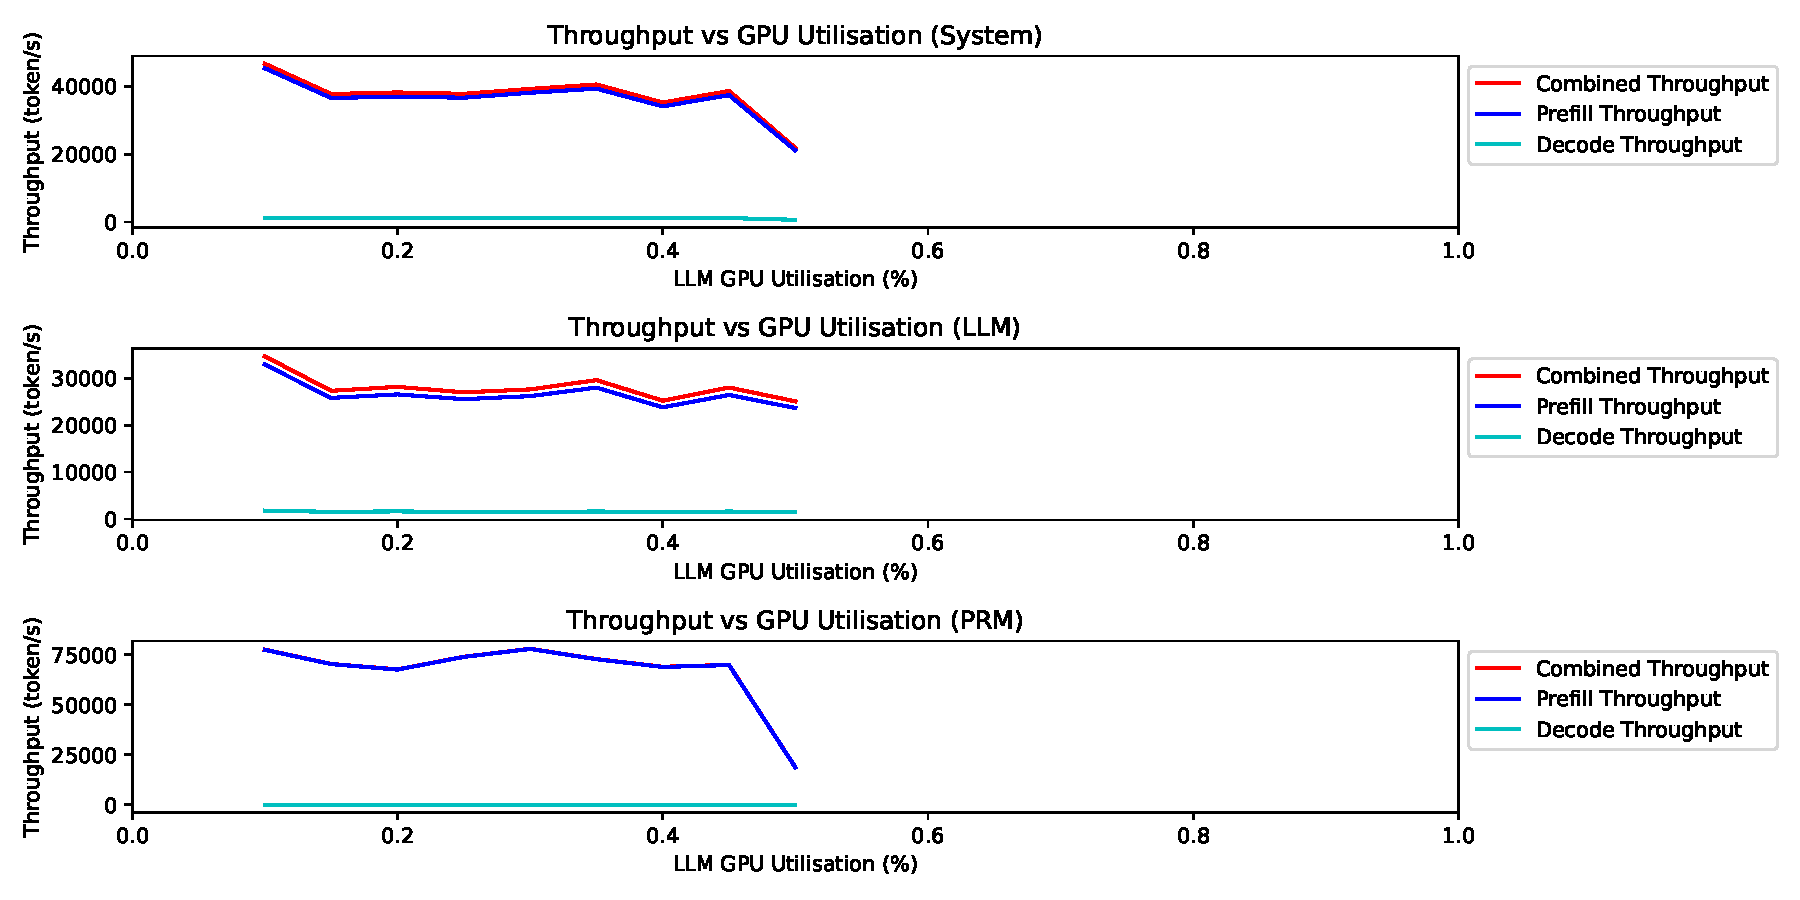
\includegraphics[width=\textwidth]{figures/system_throughput_gpu_utilisation.pdf}
  \caption{Impact on overall system throughput of varying the split in GPU memory between LLM and PRM.}
  \label{fig:system_throughput_gpu_utilisation}
\end{figure}

We can see in \ref{fig:system_throughput_gpu_utilisation} that overall system throughput peaks when the \texttt{gpu\_model\_utilization} parameter is set to 0.3, which we adopt as the baseline configuration for performance comparisons.

At the lower bound of GPU memory allocation, PRM throughput degrades significantly, leading to a corresponding drop in overall system performance. 
To investigate this behavior, we analyze throughput in terms of KV cache block allocation dynamics.

\subsection{Block Level Analysis}
%% explain what the scheduler has to do in terms of blocks for prefix caching
%% if we run out of blocks then we have to evict and recompute kv cache values

As described earlier in \ref{subsubsection:automatic_prefix_caching}, vLLM employs a KV cache manager construct to allocate and manage space in the KV cache at the granularity of fixed-size blocks. 
While the PRM is servicing requests, the KV cache manager must ensure that sufficient blocks are available to hold the corresponding KV values. 
When GPU memory is constrained, and the number of free blocks falls below demand, the KV cache manager is forced to evict existing blocks to make space for new ones. 
This eviction incurs a recomputation cost - the evicted KV values must be regenerated by re-running the corresponding prefix through the model. 
As a result, sequences relying on prefix caching no longer benefit from fast lookup and instead trigger repeated compute overhead, directly impacting throughput.

This explains the throughput degradation noted earlier and is best illustrated in figures \ref{fig:prm_block_usage_low} and \ref{fig:prm_block_usage_high}.
When the PRM is allocated less KV cache memory, it holds fewer KV cache blocks and so evictions are necessary to service requests, reducing throughput.

\begin{figure}[htbp]
  \centering
  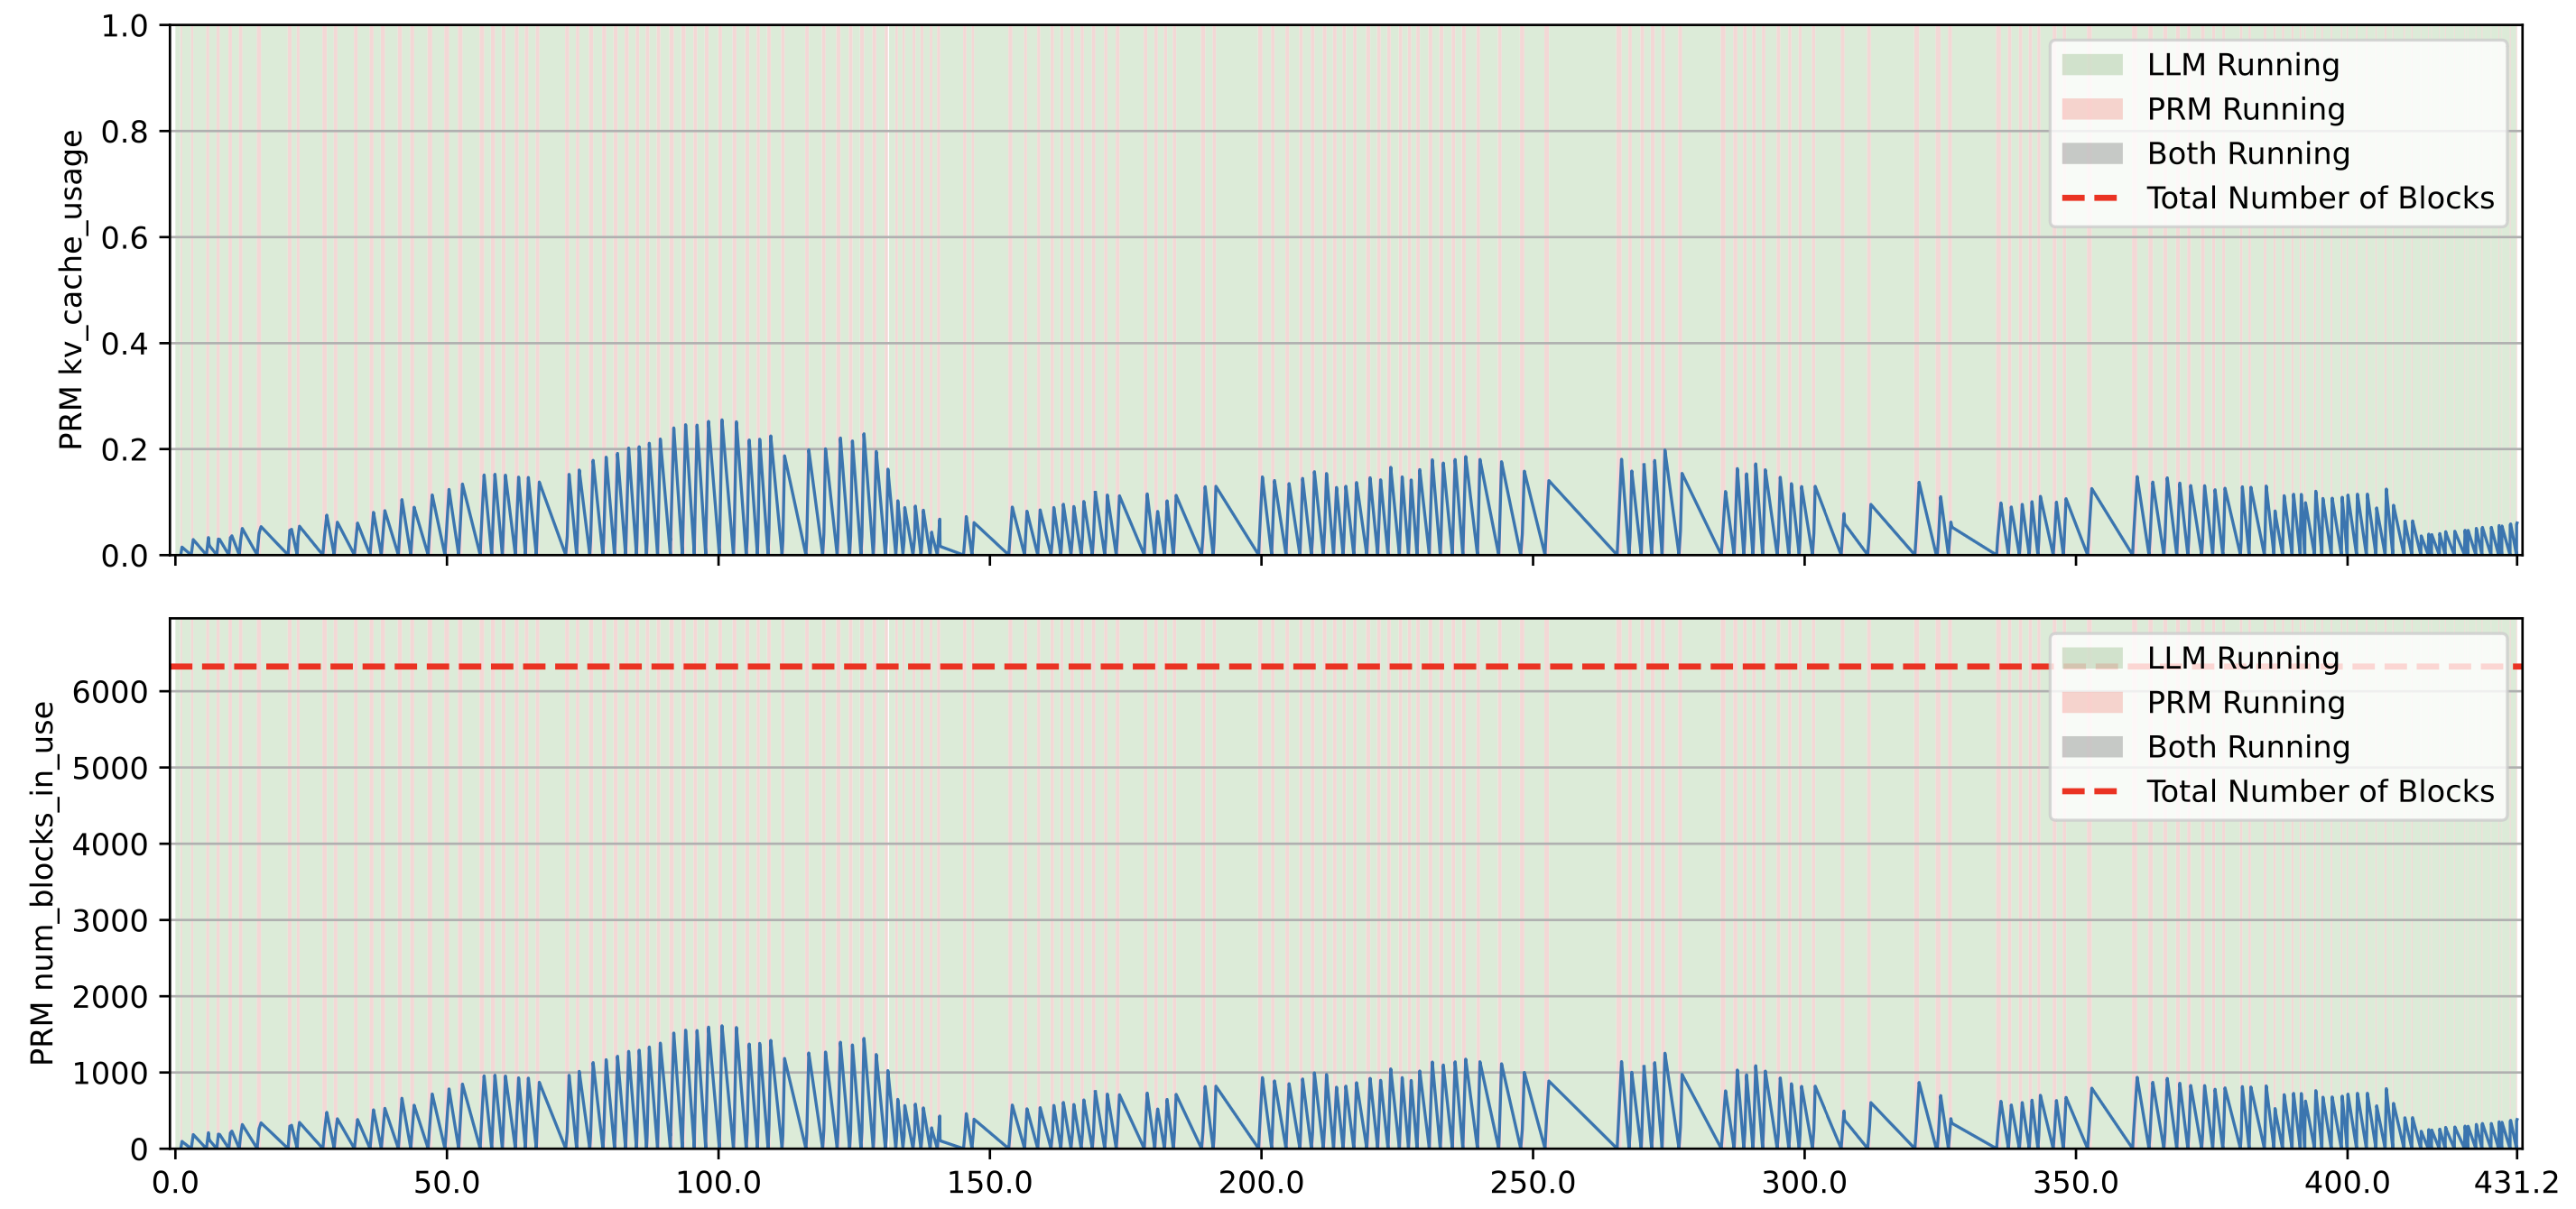
\includegraphics[width=\textwidth]{figures/prm_block_usage_low.png}
  \caption{Number of PRM KV cache blocks allocated at each scheduling step for \texttt{gpu\_model\_utilization}=0.3.}
  \label{fig:prm_block_usage_low}
\end{figure}

\begin{figure}[htbp]
  \centering
  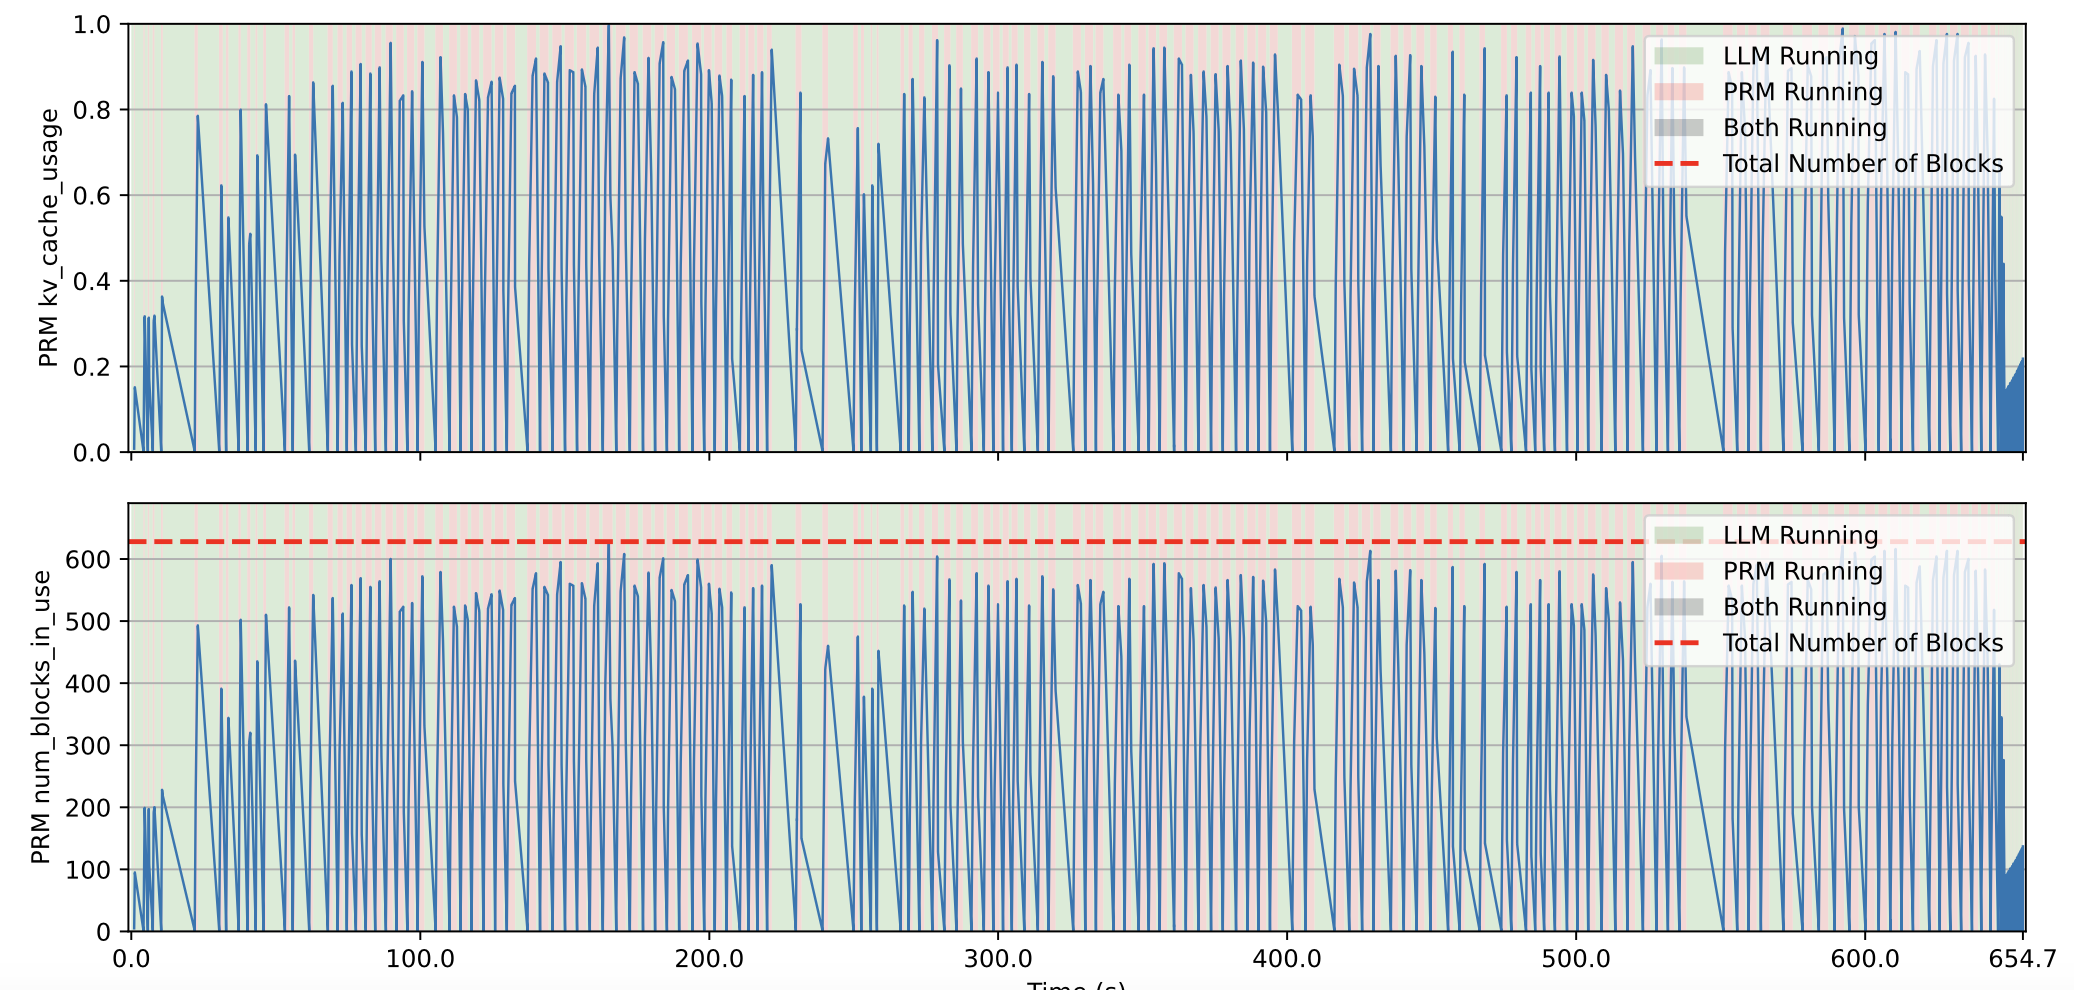
\includegraphics[width=\textwidth]{figures/prm_block_usage_high.png}
  \caption{Number of PRM KV cache blocks allocated at each scheduling step for \texttt{gpu\_model\_utilization}=0.5.}
  \label{fig:prm_block_usage_high}
\end{figure}

\chapter{KV Prefix Caching Strategy}
\begin{comment}
  - motivation
    - batch size controls gpu saturation
      - i.e bigger batches mean we are getting more useful output from a given kernel invocation
    - prefix cache rate improves performance by enabling us to reuse earlier work, thus reducing recomputation

  - we investigate how prefix cache hit rate varies as utilisation changes
    - (i guess we can also investigate how this changes as batch size/composition changes??)
  - kv cache hit rate plot
  - kv cache totals plot

  - we observe limited variability in the kv cache hit rate as we change utilisation, showing optimal access patterns for the search and learn/prm-llm use case 

  - digging into the prefix cache plots further, we check to see if any cache thrashing occurs, where we evict something that we later need
  - we can check for this by maintaining a list of all block hashes we have seen, and modify the code that checks for prefix cache hits to also check for cases where we have a prefix cache miss but for a block hash we have seen before (meaning we have previously cached it but now evicted it)

  - cache thrashing plot
    - we see that we rarely evict a block that we later need

  - conclusion, kv cache eviction policy seems well suited to our use case
    - the reason being that we create prefix cache entries for all beams, free these when we have evaluated everything, so they can all be potentially evicted. when we then call the llm/prm again for the next set of nodes, we will get prefix cache hits for all the blocks that reuse an old beam (so we won't evict these blocks) and the blocks for beams that we no longer search through will still be free and good eviction candidates. since we never revisit an old beam, we never need these blocks again so it is okay to evict them!
      - maybe include diagram justifying this
\end{comment}
Efficient use of the GPU during inference relies on two complementary strategies - maximizing compute saturation and minimizing redundant computation. 
Batch size directly affects GPU utilisation - larger batches enable more parallelism and ensure each kernel invocation does more useful work per unit time. 
At the same time, reducing redundant computation via KV cache reuse is critical to maintaining high throughput in tree-search systems like ours where prefix reuse is common.
High prefix cache hit rates avoid recomputation of the tokens in these shared prefixes while freeing up compute for new inference work.

To that end, we examine how prefix cache hit rates vary with different settings of \texttt{gpu\_model\_utilization}.

\section{Cache Hit Rates}
\begin{figure}[htbp]
\centering
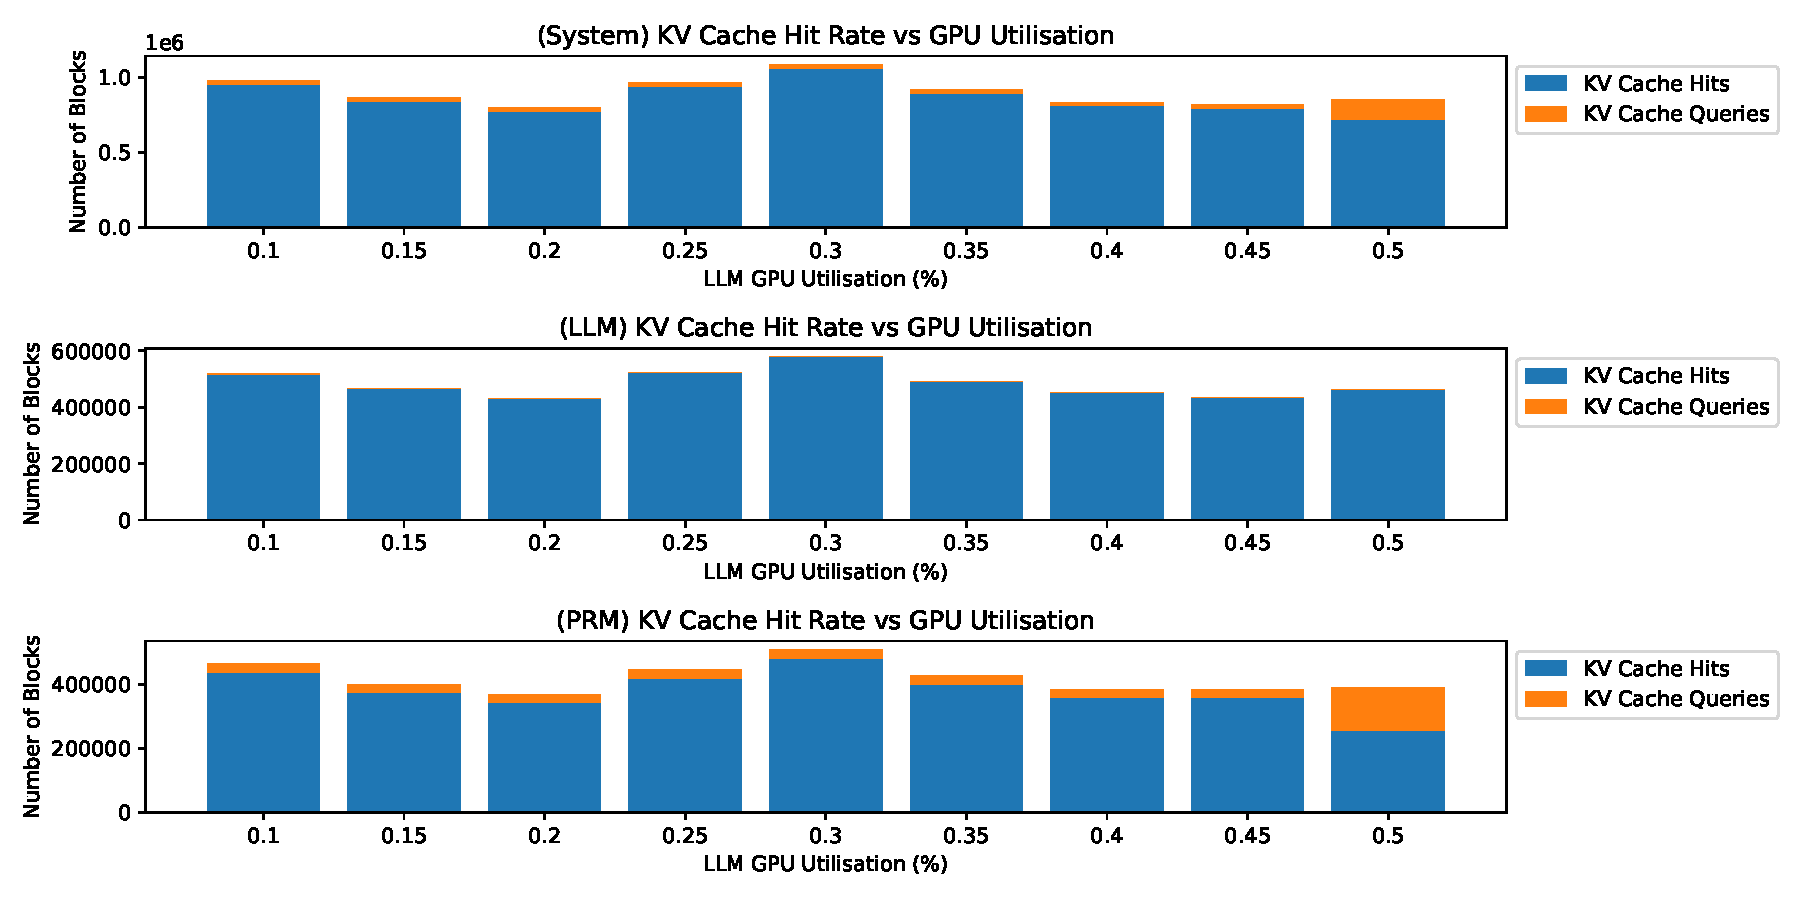
\includegraphics[width=\textwidth]{figures/kv_cache_hit_rate.pdf}
\caption{KV prefix cache hit of both the LLM and PRM across various gpu utilisation splits.}
\label{fig:kv_cache_hit_rate}
\end{figure}

Figure \ref{fig:kv_cache_hit_rate} shows that the prefix cache hit rate remains high across a wide range of utilisation levels, indicating stable reuse behavior despite memory pressure. 
This suggests that the access patterns inherent in our joint LLM-PRM search space exploration are well suited to vLLM's existing eviction policy - prefixes are reused frequently and close in time to when they were first cached.

\section{Cache Thrashing}
To further evaluate whether the existing vLLM eviction policy causes performance regressions, we analysed cache thrashing - cases where a prefix block is evicted and later needed again, resulting in a recomputation that could have been avoided. 
To detect this, we modified vLLM's KV cache manager code (see Algorithm \ref{alg:cachethrashingdetection}) to maintain a global set of seen KV block hashes. 

\begin{algorithm}[H]\label{alg:cachethrashingdetection}
\caption{Detecting Cache Thrashing in vLLM}
\begin{algorithmic}[1]
\State \textbf{Global variables:}
\State \quad \texttt{SeenBlocks} $\gets$ empty hash set
\State \quad \texttt{CacheBlocks} $\gets$ hash set of KV blocks currently in GPU memory
\State \quad \texttt{ThrashCount} $\gets$ 0
\Function{ProcessBlock}{\texttt{block\_hash}}
  \If{\texttt{block\_hash} $\notin$ \texttt{SeenBlocks}}
    \State \texttt{SeenBlocks.add(block\_hash)} \Comment{First time seeing this block}
  \Else
    \If{\texttt{block\_hash} $\notin$ \texttt{CacheBlocks}}
      \State \texttt{ThrashCount} $\gets$ \texttt{ThrashCount} + 1 \Comment{Block was evicted and reused}
    \EndIf
  \EndIf
  \State \texttt{CacheBlocks.add(block\_hash)} \Comment{Mark block as active in cache}
\EndFunction
\end{algorithmic}
\end{algorithm}

On each prefix cache miss, we check whether the block has been seen before but is no longer present in memory. 
If so, this indicates a missed opportunity for reuse due to eviction.

\begin{figure}[htbp]
\centering
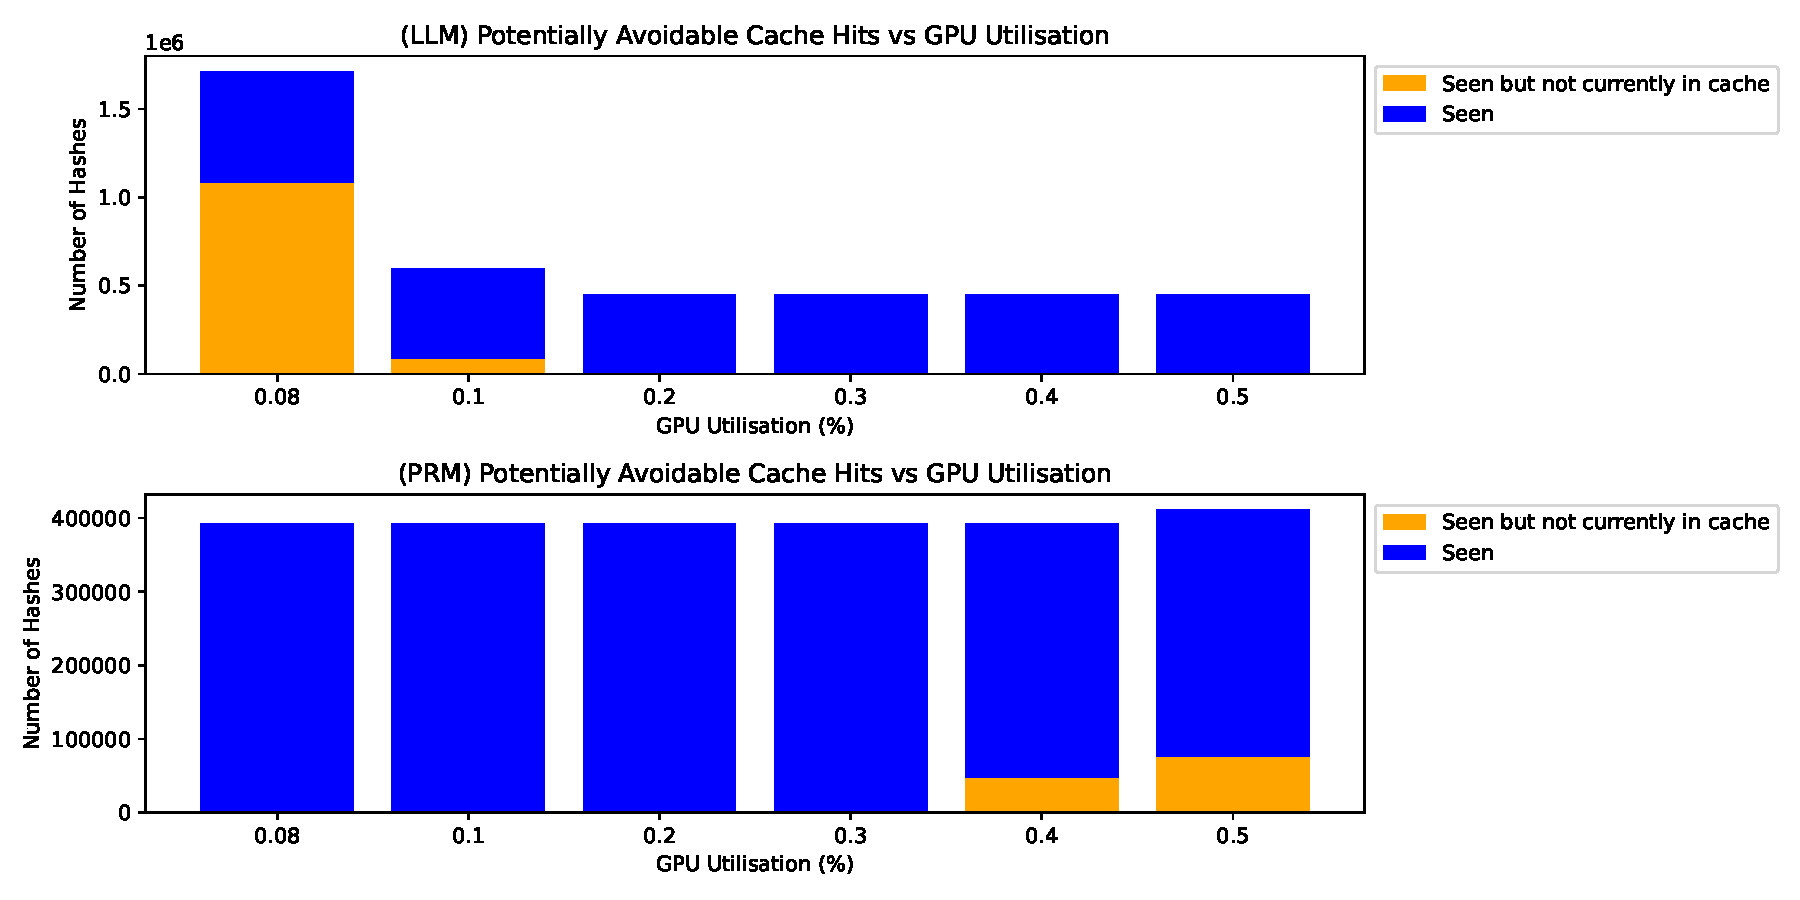
\includegraphics[width=\textwidth]{figures/kv_thrashing_stats.pdf}
\caption{Frequency of prefix cache thrashing events across utilisation levels.}
\label{fig:cache_thrashing}
\end{figure}

As shown in Figure \ref{fig:cache_thrashing}, such thrashing events are extremely rare. 

This confirms that vLLM's existing eviction policy is well matched to the temporal reuse patterns of our workload.
This tightly scoped reuse window, with cache entries being reused immediately in the next search step or not at all, explains why cache thrashing is rare and why the current eviction policy performs so well. 
Overall, our results indicate that prefix caching and memory management in our system are highly aligned with the needs of search-based multi-model inference workloads.

\chapter{Decoupled Tree Exploration}
Here we explain our decoupled tree exploration optimisation.
We detail its design, the rationale behind it and how it can be implemented into our current beam search problem setting.

\section{Motivation}
Modern LLM systems exhibit markedly different scaling behaviours across the prefill and decode stages. 
Prefill stages are largely compute-bound, driven by intensive matrix multiplications that fully utilise GPU arithmetic units. 
In contrast, decode stages, where only a single token is processed at a time, rarely saturate GPU compute capacity. 
Instead, the bottleneck shifts to memory bandwidth, as KV cache entries must be fetched and updated token by token. 
This fundamental discrepancy leads to divergent scaling dynamics and motivates different batching strategies for each phase.

To understand how these dynamics play out in practice, we analyse the composition of LLM and PRM workloads and experimentally validate the scaling behaviour of each model in isolation. 
Existing work has shown that decode throughput can be substantially improved by increasing batch size \cite{agrawal2024taming}, and we test whether this applies in our setting.

We begin by examining how many tokens are scheduled per request in LLM and PRM batches. 
To do this, we run a standard beam search workflow and record the token composition of each batch issued by the scheduler - the component responsible for determining how many tokens each request should generate. 
We then construct a histogram showing the number of tokens scheduled per request (see Figure \ref{fig:batch-hist-comparison}). 
For the LLM, this histogram reveals a sharp long tail of requests scheduling only a single token, which is typical of decode steps. 
Conversely, the PRM shows a more evenly distributed mix of token lengths, with many requests scheduling more than one token, but fewer concentrated at exactly one. This suggests partial or complete prefill.

\begin{figure}[htbp]
\centering
\subfigure[Histogram of number of tokens scheduled per request within an LLM batch.]{
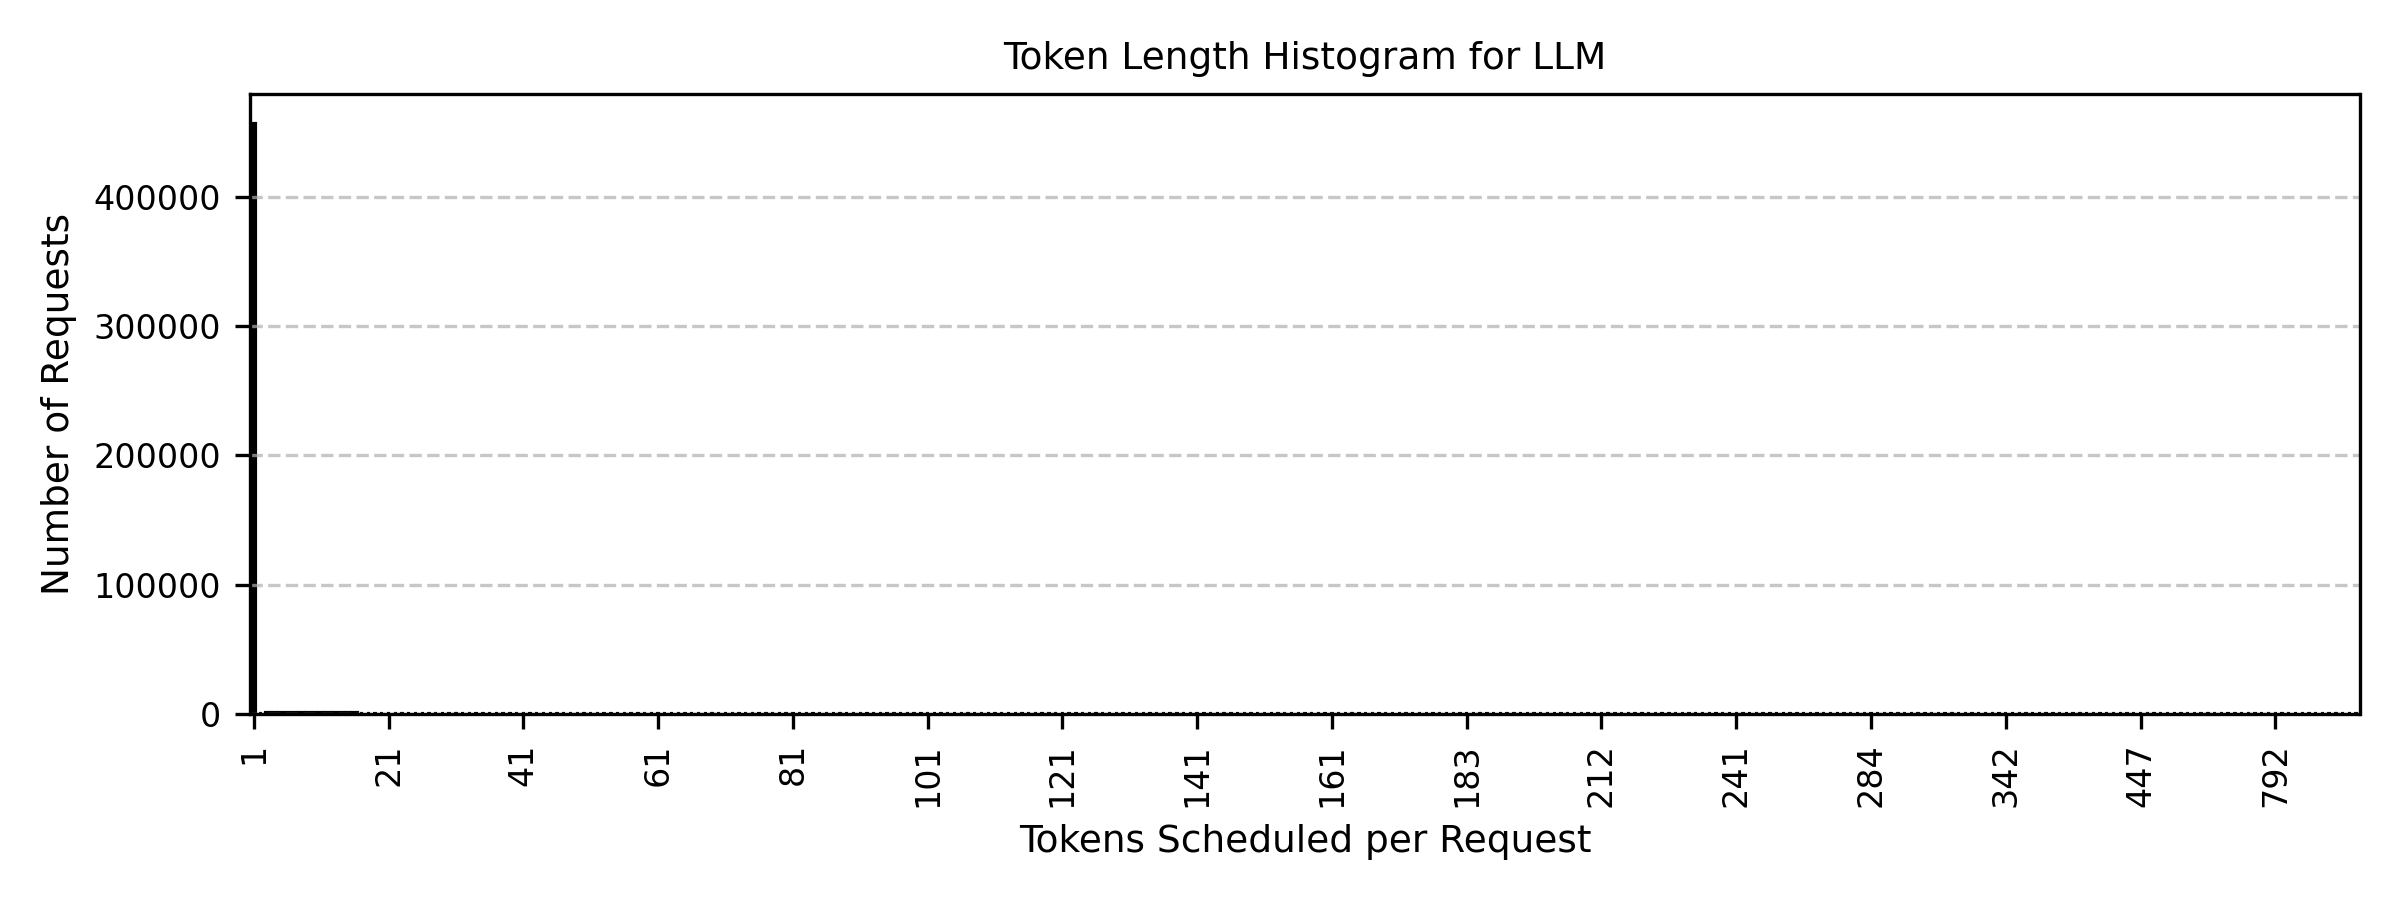
\includegraphics[width=\textwidth]{figures/LLM_tokens_scheduled_hist.png}
\label{fig:batch-hist-llm}
}
\vspace{1em}
\subfigure[Histogram of number of tokens scheduled per request within a PRM batch.]{
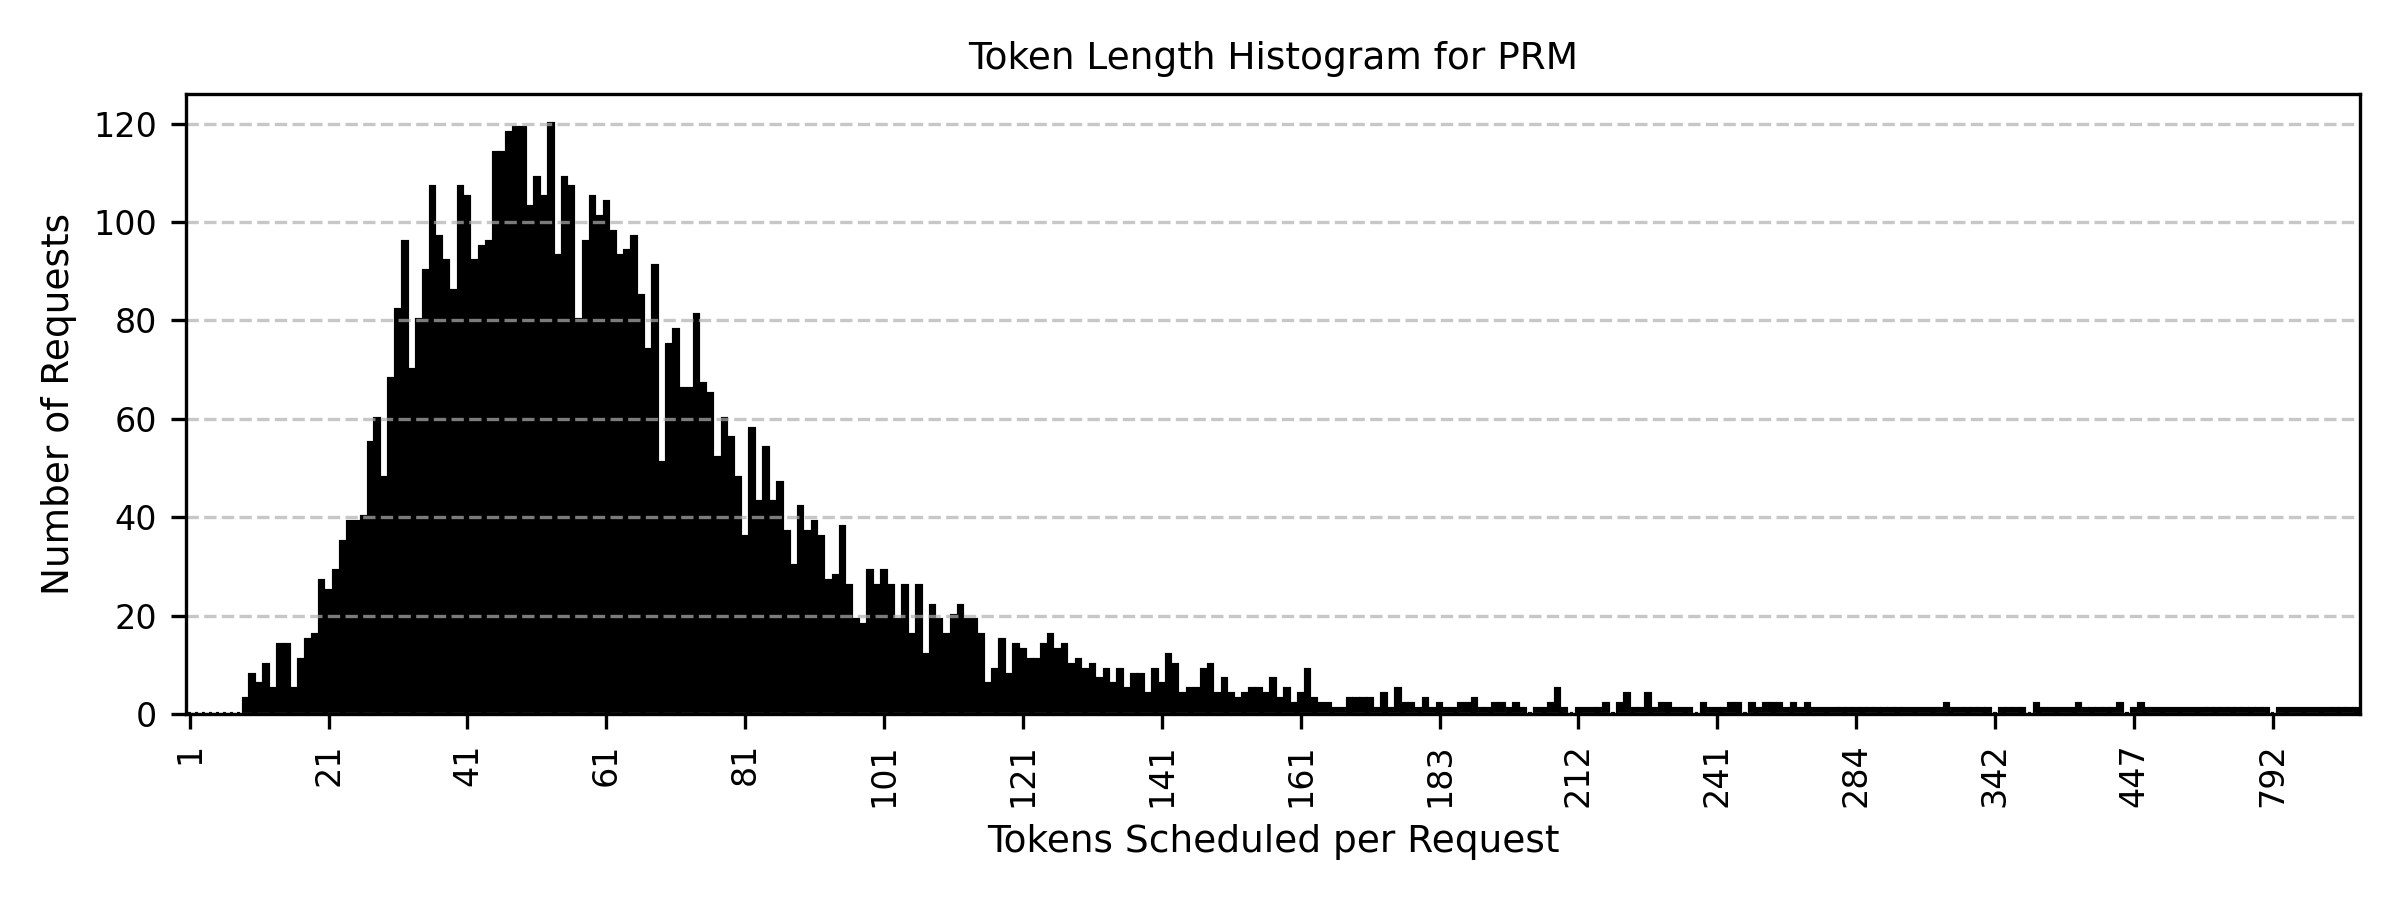
\includegraphics[width=\textwidth]{figures/PRM_tokens_scheduled_hist.png}
\label{fig:batch-hist-prm}
}
\caption{LLM batches are predominantly decode-oriented, as shown by the high frequency of 1-token requests. PRM batches exhibit a broader distribution due to their prefill-heavy workload.}
\label{fig:batch-hist-comparison}
\end{figure}

With this in mind, we isolate each model to explore how their throughput responds to increasing batch sizes. 
We vary the \texttt{max\_num\_batched\_tokens} parameter in vLLM, which controls the upper bound of tokens scheduled in a batch. 
To ensure realistic inputs, we replay prompts and responses from a previous beam search run. 
These are then fed in bulk to vLLM's generate() API, guaranteeing that the scheduler has ample tokens available to fill batches up to the configured maximum. 
Throughput is then measured in both prompts per second and tokens per second.

\begin{figure}[htbp]
\centering
\subfigure[The impact of varying LLM batch size on throughput.]{
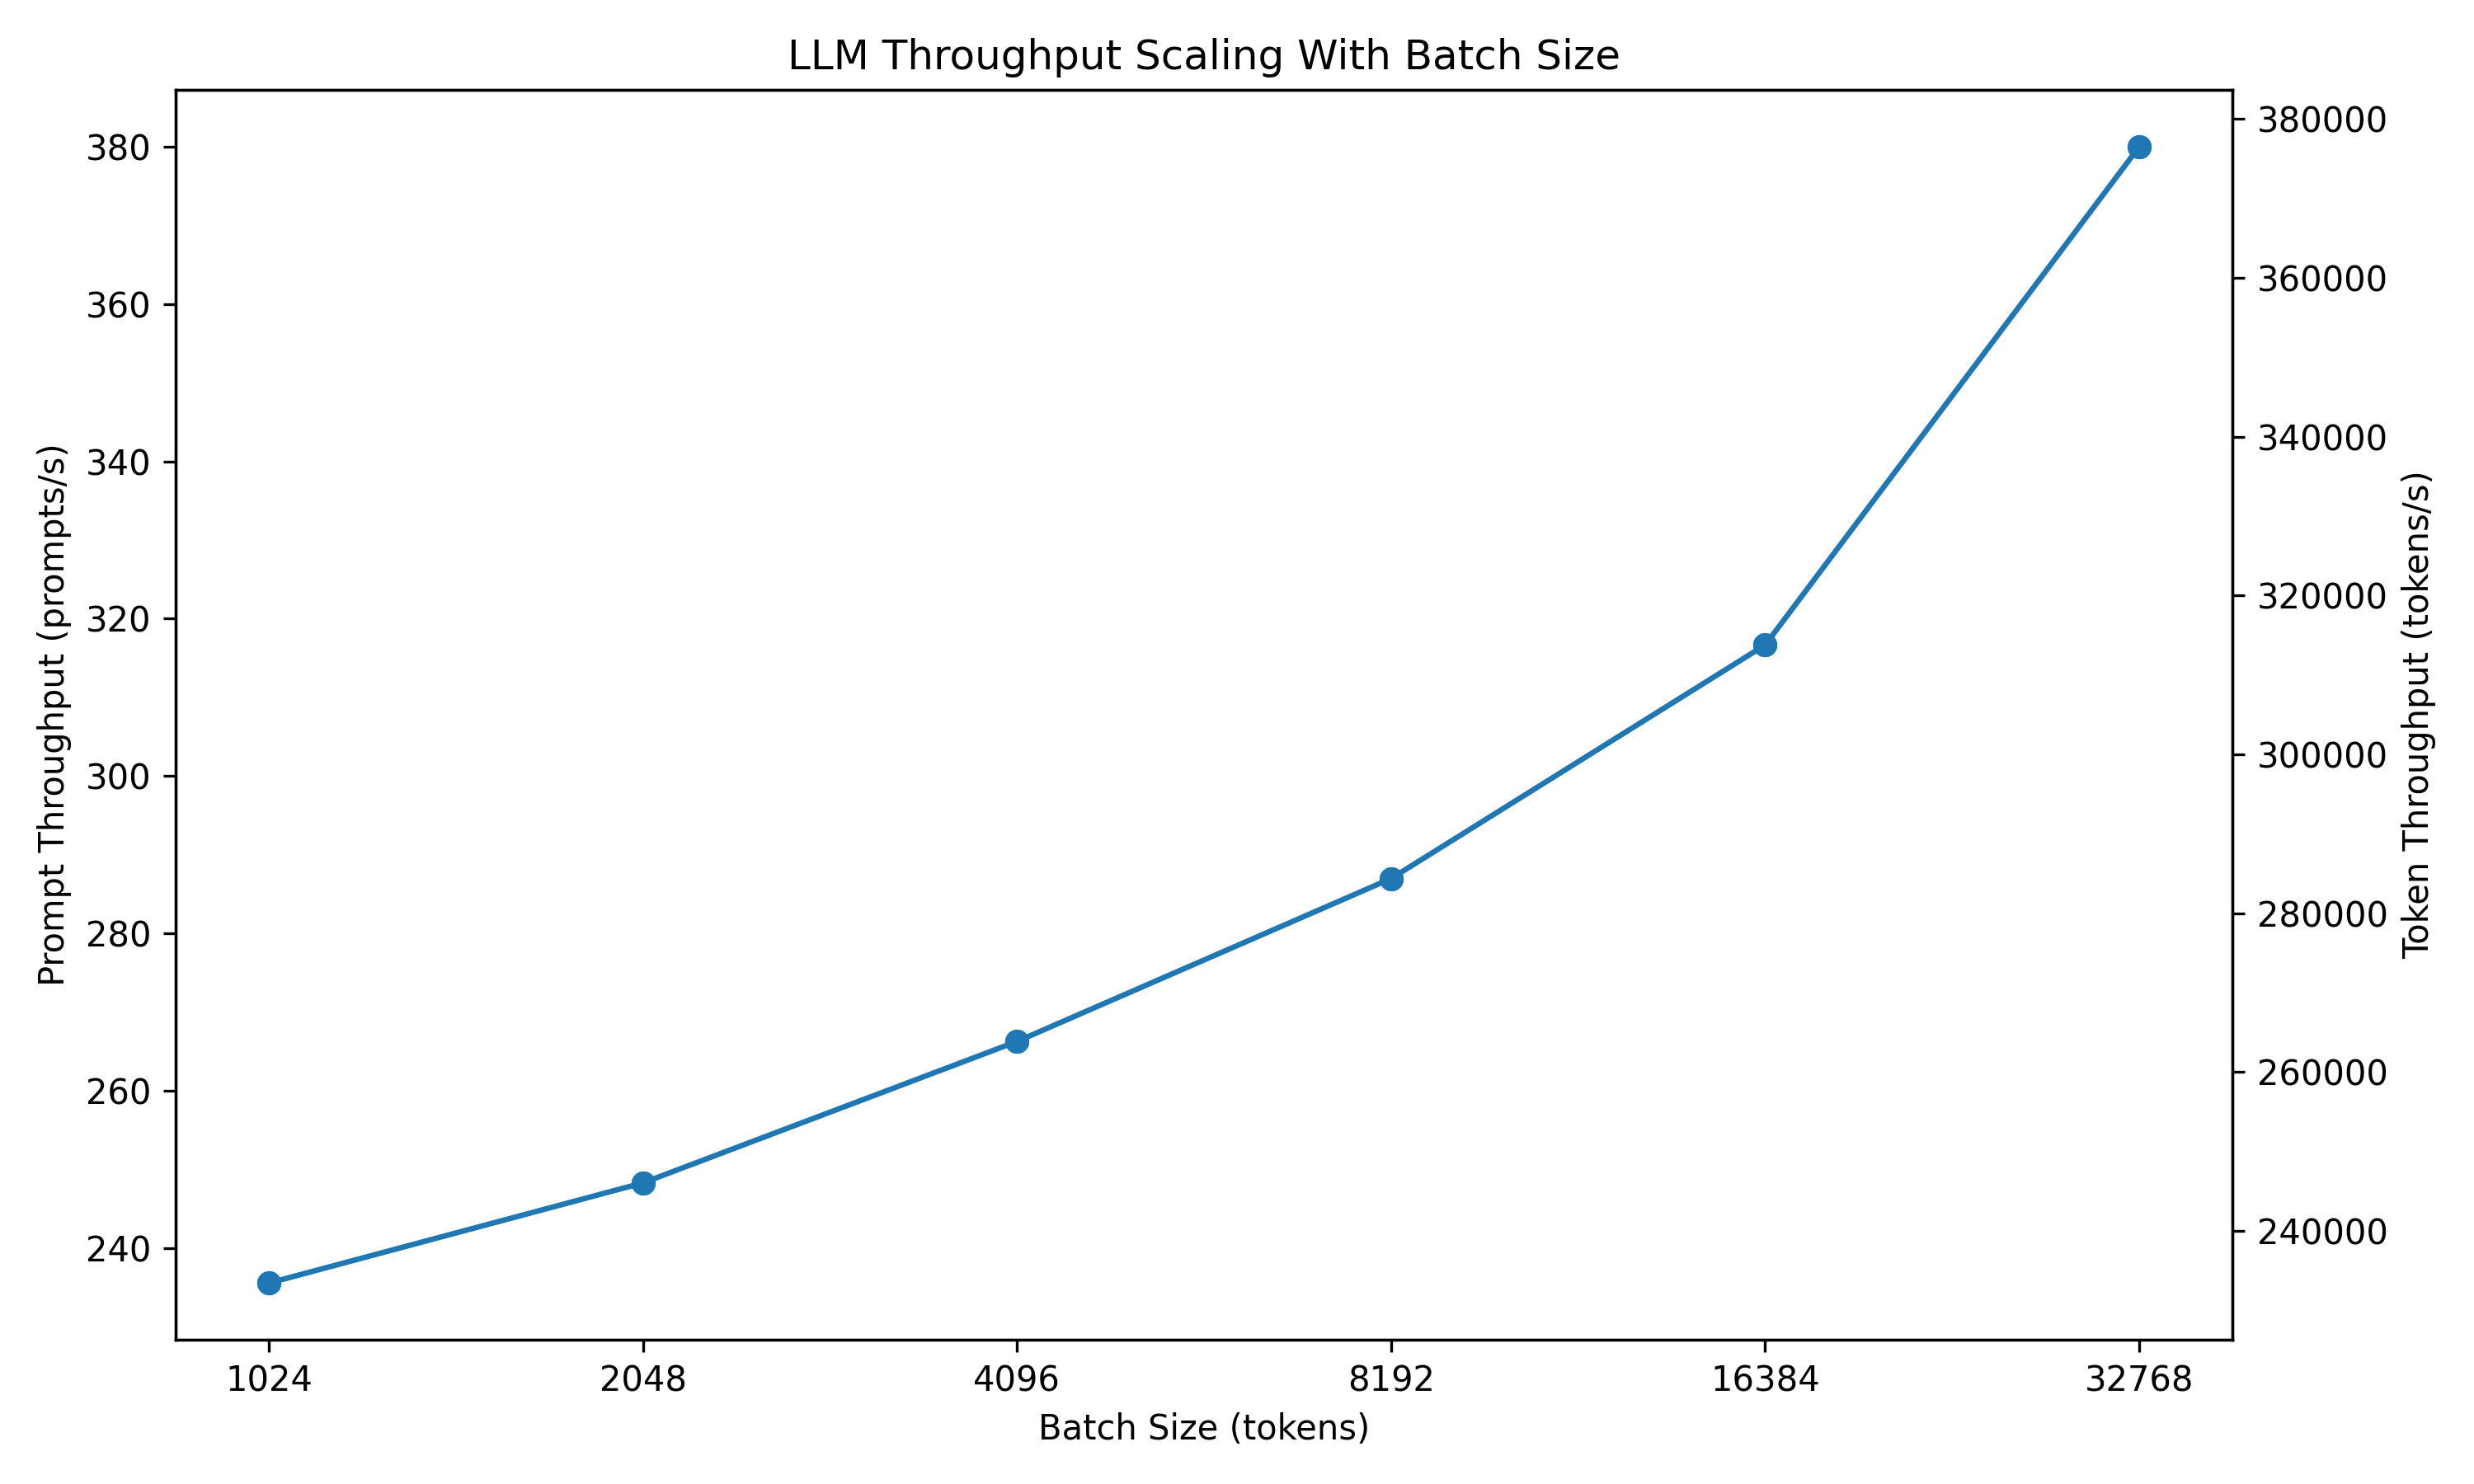
\includegraphics[width=0.45\textwidth]{figures/llm_throughput_graph.png}
\label{fig:llm_throughput_with_batch_size}
}
\hfill
\subfigure[The impact of varying PRM batch size on throughput.]{
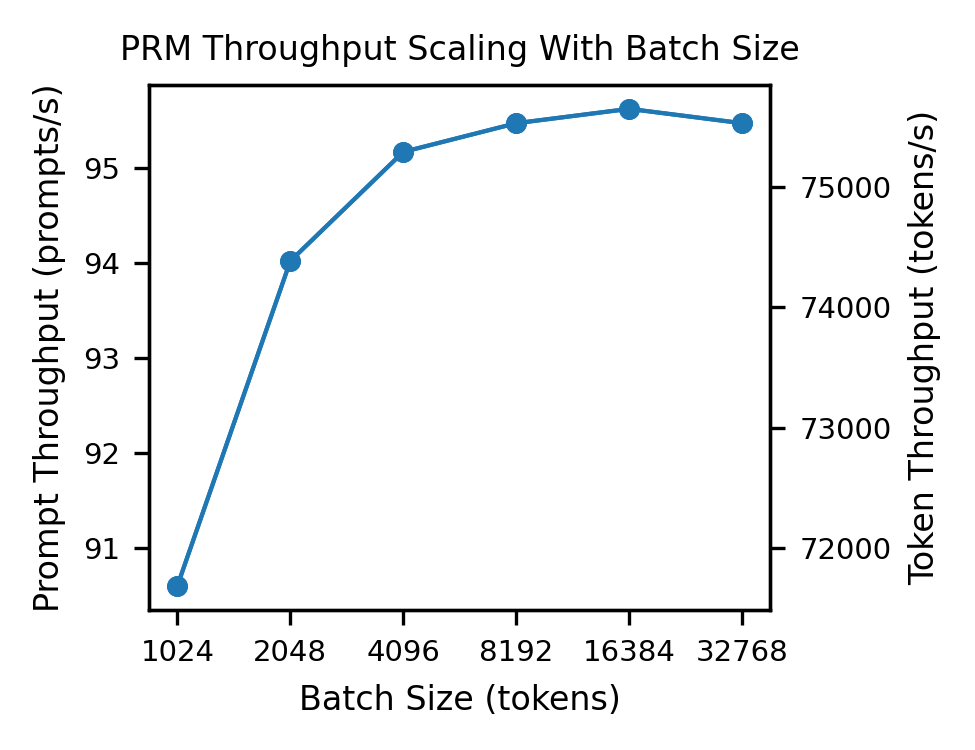
\includegraphics[width=0.45\textwidth]{figures/prm_throughput_graph.png}
\label{fig:prm_throughput_with_batch_size}
}
\caption{LLM throughput scales with batch size due to memory-bound decode efficiency. PRM throughput plateaus, constrained by the compute-bound prefill workload.}
\label{fig:prm_throughput_vs_llm_throughput}
\end{figure}

As expected, we observe a sharp increase in throughput (see Figure \ref{fig:prm_throughput_vs_llm_throughput}) for the LLM as batch size increases, confirming that decode efficiency improves with parallelism. 
In contrast, the PRM's throughput shows early saturation, with limited gains beyond a moderate batch size. 
This reinforces the idea that aggressively batching LLM decode tokens is a promising path to improved performance. 
The case strengthens further when we profile batch utilisation in a real workflow and observe that the LLM frequently submits under-filled batches.

\begin{figure}[htbp]
\centering
\subfigure[Batch utilisation histogram for LLM]{
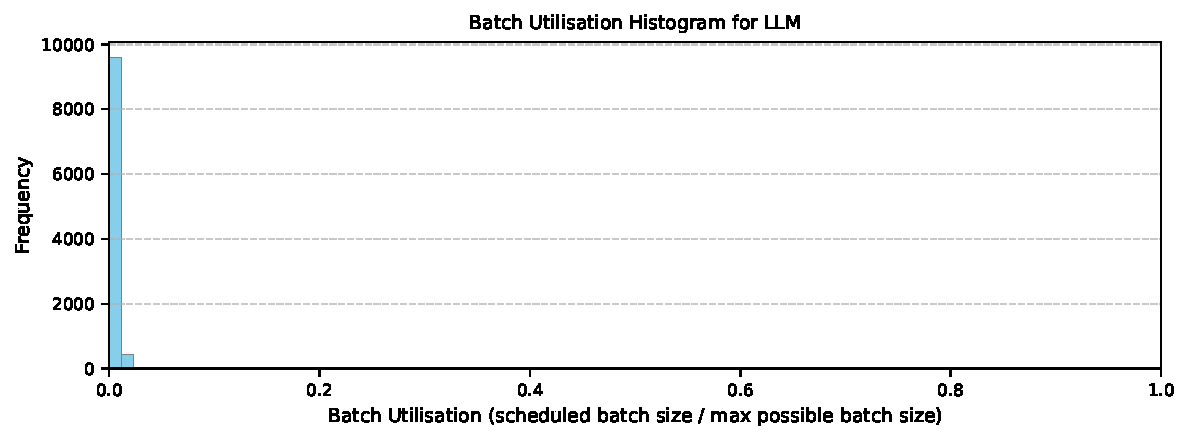
\includegraphics[width=\textwidth]{figures/LLM_batch_utilisation.pdf}
\label{fig:batch-util-llm}
}
\vspace{1em}
\subfigure[Batch utilisation histogram for PRM]{
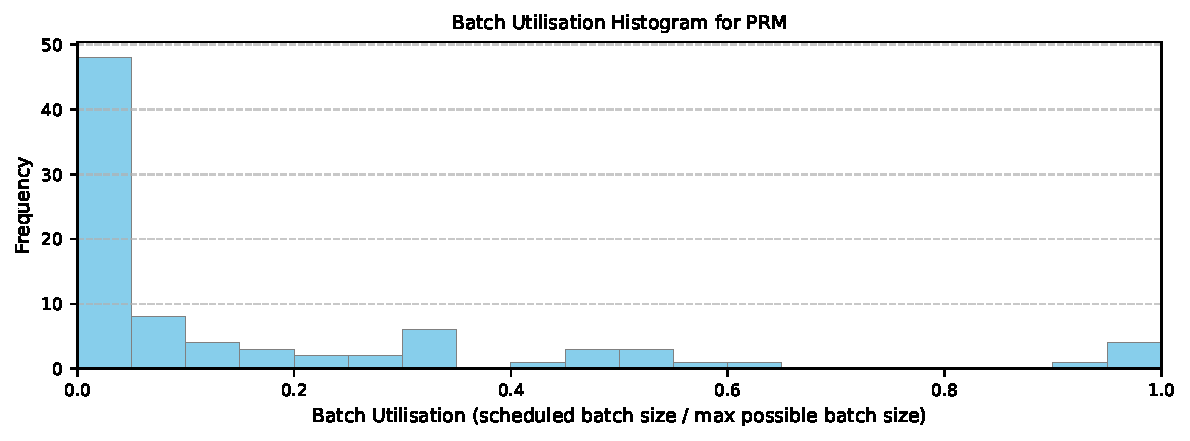
\includegraphics[width=\textwidth]{figures/PRM_batch_utilisation.pdf}
\label{fig:batch-util-prm}
}
\caption{LLM batch utilisation is frequently suboptimal, with many invocations well below the scheduler’s maximum capacity.}
\label{fig:batch-utilisation-comparison}
\end{figure}

Additionally, many LLM decode batches are under-filled - that is, they schedule far fewer tokens than the model could process in a single step. 
This underutilisation reflects a tight coupling between the LLM and PRM, where the LLM can only generate tokens once the PRM has fully evaluated and selected nodes. 
This introduces serial bottlenecks and leaves LLM compute capacity idle.

These observations motivate a decoupled search strategy, where the LLM and PRM operate semi-independently. 
Rather than waiting for the PRM to determine which nodes to expand next, the LLM can opportunistically generate additional tokens - either for unexplored nodes within the same problem or from unrelated queued requests. 
This allows us to improve LLM throughput by better saturating batches, even if some of the work may later be discarded.

Two strategies emerge:
\begin{itemize}
  \item \textbf{Eager Scheduling:} The LLM proactively generates tokens for nodes that we are certain will be used later, such as expansions from other active requests in the queue. 
    The key benefit is that all generated tokens are guaranteed to be useful. 
    However, there are trade-offs. 
    Prefill may be required for unrelated requests, and prefill is significantly more expensive than decode. 
    In addition, different problems are unlikely to share KV cache blocks, so this can increase cache contention and lead to unnecessary evictions.
  \item \textbf{Speculative Expansion:} Here, the LLM begins generating tokens for nodes that have not yet been selected by the PRM. 
    If the PRM later chooses to expand these nodes, we avoid latency by reusing work already done. 
    This allows us to increase current LLM batch size and potentially improve throughput. 
    However, speculative work carries the risk of being wasted if the PRM selects a different path, and it may increase memory pressure due to added cache entries.
\end{itemize}

In both cases, increased KV cache fragmentation and pressure may become limiting factors. 
Since prefill-heavy speculative generations may evict high-value decode paths, understanding the runtime impact on the KV cache remains an important area for future profiling and optimisation.

In summary, the mismatch in prefill and decode scaling, combined with frequent underutilisation of LLM batches, highlights a missed opportunity in tightly coupled LLM–PRM workflows. 
Decoupling the LLM from the PRM allows the LLM to independently explore alternative nodes, whether by speculating within the same search tree or by pulling in work from other queued problems. 
This decoupling means that the LLM and PRM no longer operate on the exact same nodes at each step, enabling better batch saturation and throughput, and reducing end-to-end latency - even if it comes at the cost of some wasted computation or cache pressure.

\section{Design}
\begin{comment}
With decoupled tree exploration, we aim to take advantage of the dynamics in throughput scaling between the decode-heavy LLM and the prefill-heavy PRM in order to fill a scheduling step in the LLM with more useful work.
In particular, because decode throughput increases with greater batch size, we increase the batch size of the LLM by packing it with tokens from other requests and, in the event that there are no other requests to process, we speculatively explore other nodes in the search tree.
Speculative exploration enables us to include potentially useful work in a batch - if the PRM decides that a particular beam is worth exploring, then we may have already expanded this node and so have managed to avoid the overhead incurred by scheduling another kernel execution were we to expand the beams sequentially.

Doing this decouples the search space exploration strategy between the LLM and PRM, with both models processing tokens for different parts of the tree at each generation step.
This is accomplished by maintaining a queue of work for both the LLM and PRM, with each model popping off work from this queue on invocation (see \ref{alg:treesearchalgorithm}).

We use a \textsc{Beam} data structure to manage the state of a beam during exploration - ensuring we can keep track of any reasoning steps that we have speculatively expanded (see \ref{alg:datastructures}).
We do this through the use of a \texttt{last\_scored\_thought} attribute that 
The PRM should only ever score the next thought occuring after the \texttt{last\_scored\_thought} index.
Scoring any thoughts after this represents potentially needlessly wasted computation by the PRM: since the PRM batch size is smaller than that of the LLM and there is a data dependency from the PRM on the LLM, there always exists useful work to do by the PRM.
We encapsulate these reasoning steps within a \textsc{Thought} data structure that store the associated PRM score of the step (see \ref{alg:datastructures}).

As a result of the different batch sizes between the PRM and LLM, they each have different policies for selecting what work to include in their input batch. 
These policies are outlined in \ref{alg:llmtreesearch} and \ref{alg:prmtreesearch}. 
The LLM prioritises generating reasoning steps for nodes that have been recently scored and deemed to be worthwhile paths to continue exploring, before scheduling work from other waiting problems in order to fill up its input batch.
It only speculatively explores nodes if it still cannot fill up its input batch.
The PRM only scores the shallowest nodes in the tree - it never scores a speculatively decoded reasoning step.
\end{comment}

In decoupled tree exploration, we aim to exploit differences in throughput dynamics between the decode-bound LLM and the prefill-bound PRM. 
The key idea is to maximise LLM utilisation during each scheduling step by filling its batch with useful work. 
Since LLM decoding throughput improves with larger batch sizes, we increase the LLM’s batch size by packing it with tokens from multiple requests. 
If no additional requests are available, we opportunistically expand speculative nodes in the current search tree.

This speculative exploration allows the LLM to perform potentially useful computations ahead of time. 
If the PRM later determines that a beam is worth pursuing, we may already have generated its child nodes-thereby avoiding the cost of launching another generation step. 
This strategy effectively overlaps the LLM’s generation work with the PRM’s slower scoring, improving overall throughput.

Crucially, this approach decouples the search space traversal performed by the LLM and PRM. 
Rather than both models operating synchronously on the same node, they each work on different parts of the tree at any given generation step. 
This is implemented by maintaining separate work queues for the LLM and PRM. Each model consumes work from its respective queue upon invocation (see Algorithm \ref{alg:treesearchalgorithm}).

\begin{algorithm}[H]\label{alg:treesearchalgorithm}
\caption{Decoupled Tree Search Algorithm} 
\begin{algorithmic}[1]
\State Initialise list of beams $\mathcal{B} = \{B_1, B_2, \dots, B_n\}$ with associated problems
\State Initialise empty request queue $\mathcal{Q}_{\text{Req}}$
\State Initialise empty LLM prompt queue $\mathcal{Q}_{\text{LLM}}$
\State Initialise empty PRM scoring queue $\mathcal{Q}_{\text{PRM}}$
\State Set LLM and PRM batch sizes: $N_{\text{LLM}}, N_{\text{PRM}}$
\While{any beam in $\mathcal{B}$ is active (not pruned or completed)}
    \State \textbf{SelectLLMPrompts()}
    \State \textbf{GenerateLLMOutputs()}
    \State \textbf{ProcessLLMResults()}
    \State \textbf{SelectPRMBatch()}
    \State \textbf{GeneratePRMOutputs()}
    \State \textbf{ProcessPRMResults()}
    \State \textbf{PruneBeamsUsingScores()}

    \For{each beam $B \in \mathcal{B}$}
      \If{$B.\text{pruned}$ or $B.\text{completed}$}
        \State Remove $B$ from $\mathcal{B}$
      \EndIf
    \EndFor
\EndWhile
\end{algorithmic}
\end{algorithm}

To track progress through the tree, we use a \textsc{Beam} data structure, which manages the state of each active beam. 
This includes recording any reasoning steps that have been speculatively expanded by the LLM (see Algorithm \ref{alg:datastructures}). 
Each \textsc{Beam} maintains a \texttt{last\_scored\_thought} index, indicating which thoughts have been confirmed by the PRM. 
The PRM is only permitted to score the thought immediately following this index; scoring beyond it would represent unnecessary computation, as these thoughts may be speculative and ultimately pruned. 
Given that the PRM’s batch size is smaller and it depends on LLM outputs, its capacity is best used on work that is guaranteed to be relevant.

Individual reasoning steps are represented by the \textsc{Thought} data structure, which stores both the LLM-generated text and (optionally) the PRM-assigned score (see Algorithm \ref{alg:datastructures}).

\begin{algorithm}[H]\label{alg:datastructures}
\caption{Beam Search Data Structures}
\begin{algorithmic}[1]
\State \textbf{Structure} \textsc{Thought}:
\State \hspace{0.5cm} \texttt{text}: String \Comment{The content of the thought}
\State \hspace{0.5cm} \texttt{score}: Float or \texttt{None} \Comment{Score assigned by PRM}
\State \hspace{0.5cm} \texttt{stop\_reason}: String or \texttt{None} \Comment{Why generation stopped, e.g., ``EOS''}

\Statex

\State \textbf{Structure} \textsc{Beam}:
\State \hspace{0.5cm} \texttt{problem}: String \Comment{The original problem prompt}
\State \hspace{0.5cm} \texttt{thoughts}: List of \textsc{Thought} \Comment{The search tree branch}
\State \hspace{0.5cm} \texttt{last\_scored\_thought}: Integer \Comment{Index of last thought scored by PRM}
\State \hspace{0.5cm} \texttt{pruned}: Boolean \Comment{Whether the beam has been pruned}
\State \hspace{0.5cm} \texttt{completed}: Boolean \Comment{Whether the beam has reached a stopping condition}
\end{algorithmic}
\end{algorithm}

Because the LLM and PRM operate under different batch size constraints, they follow distinct scheduling policies for selecting work. 
These are detailed in Algorithms \ref{alg:llmtreesearch} and \ref{alg:prmtreesearch}. 
The LLM prioritises expanding nodes that were recently scored and found to be promising. 
If its batch is not full, it then considers work from other pending problems. 
Only as a last resort does it generate speculative continuations. 
In contrast, the PRM only scores the shallowest unscored node in each beam, and never scores speculative reasoning steps.

\begin{algorithm}[H]\label{alg:llmtreesearch}
\caption{LLM Tree Exploration Strategy}
\begin{algorithmic}[1]
\Statex \textbf{Select LLM Prompts:}
\State $\mathcal{Q}_{\text{LLM}} \gets [\,]$


\For{each beam $B \in \mathcal{B}$} \Comment{Process currently running beams first}
  \If{$B.\text{last\_scored\_thought} < |B.\text{thoughts}|$}
      \State \textit{// PRM still catching up; wait before expanding}
      \State \textbf{continue}
  \EndIf

  \State Select most recent thought $t$
  \State Generate prompt for expanding $t$, append to $\mathcal{Q}_{\text{LLM}}$
\EndFor

\If{$|\mathcal{Q}_{\text{LLM}}| < N_{\text{LLM}}$}
    \For{each request $R \in \mathcal{Q}_{\text{Req}}$} \Comment{Fill up batch with tokens from other queued requests first}
      \State Generate beam $B$ for request and append to $\mathcal{B}$
      \State Generate initial prompt for empty beam $B$, append to  $\mathcal{Q}_{\text{LLM}}$
      \If{$|\mathcal{Q}_{\text{LLM}}| = N_{\text{LLM}}$}
          \State \textbf{break}
      \EndIf
    \EndFor
\EndIf

\If{$|\mathcal{Q}_{\text{LLM}}| < N_{\text{LLM}}$}
    \For{each beam $B \in \mathcal{B}$} \Comment{If batch size is still too small, speculatively decode new reasoning steps}
        \If{$B$ is not pruned or completed}
            \State Select speculative thought $t$ from $B$
            \State Generate prompt to expand $t$, append to $\mathcal{Q}_{\text{LLM}}$
            \If{$|\mathcal{Q}_{\text{LLM}}| = N_{\text{LLM}}$}
                \State \textbf{break}
            \EndIf
        \EndIf
    \EndFor
\EndIf
\end{algorithmic}
\end{algorithm}

\begin{algorithm}[H]\label{alg:prmtreesearch}
\caption{PRM Tree Exploration Strategy}
\begin{algorithmic}[1]
    \Statex \textbf{Select PRM Batch:}
    \State Truncate $\mathcal{Q}_{\text{PRM}}$ to $N_{\text{PRM}}$ items
    \State Query PRM with $\mathcal{Q}_{\text{PRM}}$, get scored thoughts $\mathcal{T}_{\text{PRM}}$ \\
    \Statex \textbf{Process PRM Results:}
    \For{each scored tuple $(B, t, s) \in \mathcal{T}_{\text{PRM}}$}
        \State Set $t.\text{score} \gets s$
        \State Increment $B.\text{last\_scored\_thought}$
        \State Remove $(B, t)$ from $\mathcal{Q}_{\text{PRM}}$
    \EndFor
\end{algorithmic}
\end{algorithm}

\chapter{Evaluation}
\begin{comment}
  - bit at the start
    - we evaluate our decoupled tree exploration strategy with respect to our baseline metrics and aim to establish an estimate of how much it could improve throughput
  - potential performance improvement 
    - estimate number of requests we could potentially add to the batch
    - estimate number of beams we could speculatively expand
    - these two can give us an estimate of how the throughput could increase
      - however we also need to consider what percentage of speculative tokens will actually turn out to be useful

    - speak about how this improves llm throughput, but in a single GPU system, we are still bottlenecked by prm throughput

  - complicating factors
    - batch composition
      - if we are adding in prompts from other requests we will need to execute prefill on these, changes the composition of the batch and leads to greater inter token latency
        - graph showing latency of requests containing prefills vs decode only requests
    - kv cache pressure
      - graph showing num blocks used as a function of max_num_seqs?
        - we should hopefully see that as we add more more max num seqs the number of blocks increases - potentially leading to eviction that we saw earlier that degraded throughput
    - speculation hit rate
      - kind of hard to evaluate as it depends on how many things we are speculating for
        - if we pack our batch full of more speculation then we are more likely to get a hit
  - also comment on scheduling complexity
    - should basically be minimal given that gpu kernel invocations dominate (get some figures for this - maybe the stuff guo had)
      - basically profile time spent in different parts of the overall cycle
\end{comment}
\section{Evaluation}

We now present a prospective evaluation of our decoupled tree exploration strategy. 
Since we have not yet implemented the full optimisation, our aim here is to estimate its potential impact on throughput and system efficiency, based on measured characteristics of LLM and PRM behaviour and architectural constraints.

\subsection{Estimating Potential Gains}

Our strategy is motivated by a key mismatch: decode-heavy LLMs scale well with batch size, while prefill-heavy PRMs quickly saturate. 
Empirical profiling (see figures \ref{fig:prm_throughput_vs_llm_throughput} and \ref{fig:batch-utilisation-comparison}) confirms that the LLM is frequently underutilised due to tight coupling with the PRM. 
Decoupling allows the LLM to perform additional useful or potentially useful work by filling out its batch with:
\begin{itemize}
  \item Tokens from unrelated pending requests (eager scheduling)
  \item Speculative expansions of beams not yet selected by the PRM
\end{itemize}

We can estimate the theoretical gains in two ways:

\paragraph{Batch Size and LLM Throughput}

By adding speculative or eager tokens to the LLM batch, we aim to increase the number of tokens processed per invocation. 
Since decode throughput scales with batch size (Figure \ref{fig:llm_throughput_with_batch_size}), this improves GPU utilisation and reduces per-token latency. 
For example, if the current average LLM batch utilisation is 10\% (defined as the number of scheduled tokens divided by the batch’s maximum capacity), and we increase this to 40\% through speculative expansions, then LLM throughput could increase by up to 4$\times$ under ideal conditions.

\paragraph{Amortising Kernel Overhead via Speculation}

In standard beam search, every reasoning step must be decoded by a dedicated LLM kernel invocation. 
With our decoupled strategy, speculative or eagerly scheduled steps may be generated ahead of time and reused later - avoiding the need to schedule a new LLM invocation for them. 
This amortises kernel launch overhead across more tokens and reduces the number of kernel executions required for the same amount of useful output. 
The extent of this benefit depends on the the proportion of speculatively generated reasoning steps that are ultimately retained by the PRM - the speculation hit rate. 
For instance, if 50\% of speculative work is reused, we could cut the number of LLM invocations by up to half.

\vspace{0.5em}
Together, these effects, better batch utilisation and amortised kernel scheduling, suggest that decoupled tree exploration could significantly improve LLM throughput. 
However, as we discuss below, these gains are constrained by batch composition, cache behaviour and speculative hit rates.

\subsection{Practical Constraints and Trade-offs}

\paragraph{Batch Composition}

Packing unrelated requests into the same batch improves LLM utilisation, but it also changes batch characteristics. 
Decode-only batches are fast and memory-efficient while introducing new prompts requires prefill, which is slower and more memory intensive. 
We expect increased inter-token latency and degraded throughput in hybrid batches \ref{agrawal2024taming}. 

% plot goes here showing latency between decode only and hybrid batches

\begin{comment}
A future experiment could compare LLM latency across:
\begin{itemize}
  \item Pure decode batches
  \item Batches with queued prefill requests
  \item Batches with intra-tree speculative expansions
\end{itemize}
\end{comment}

\paragraph{Speculation Hit Rate}

The effectiveness of speculative decoding depends on the speculation hit rate - the fraction of speculative reasoning steps that are ultimately reused by the PRM.  
Higher hit rates allow more speculative work to be retained, reducing wasted compute and improving overall efficiency.  
However, the hit rate is not fixed - it varies with both beam search configuration and batch composition strategy.

In particular, hit rate increases with beam width.  
When more beams are kept alive after PRM scoring, there is a greater chance that at least one of the speculatively expanded nodes belongs to a retained path.  
This makes broader beam search more amenable to speculative decoding.

Hit rate is also influenced by how much of the LLM batch is devoted to speculative expansions versus eager scheduling.  
Eager expansions - tokens generated for queued requests we know will be used - always represent useful computation, but they reduce the number of speculative expansions that can be included in a batch.  
This in turn lowers the overall probability of a speculative hit, since fewer speculative candidates are attempted.

There is therefore a trade-off between guaranteed utility, through eager scheduling, and potential future reuse, through speculation.  
This trade-off is complicated further by the impact of batch composition on LLM latency.  
Decode-only batches, for example speculative continuations from the same search tree, tend to execute faster than hybrid batches that include new prefill prompts from unrelated problems.  
As a result, aggressively increasing eager work may reduce speculation hit rate and increase batch latency, undermining the gains from either strategy.

Quantifying this trade-off requires careful profiling of batch composition, token latency, and reuse rates.  
Future work could explore adaptive scheduling policies that dynamically balance speculation and eagerness based on runtime conditions.

\paragraph{KV Cache Pressure}
Speculative expansions and prefill introduce additional sequence entries into the KV cache. 
This increases memory pressure and may reduce the number of requests the system can handle concurrently. 
Specifically, prefill work for unrelated prompts is unlikely to reuse cache blocks significantly, increasing the number of KV cache blocks actively in use. 
Further, speculative tree expansions grow the depth of the beam search tree, again allocating more KV cache blocks.
In the event of high contention for the KV cache, blocks may be evicted, leading to recomputation of KV cache entries and reducing throughput.

%% graph showing num blocks used as a function of max_num_seqs?
%% we should hopefully see that as we add more more max num seqs the number of blocks increases - potentially leading to eviction that we saw earlier that degraded throughput

\subsection{Scheduling Complexity}
Despite adding speculative work, the core scheduling mechanism remains simple. 
LLM and PRM still run sequentially, and each model draws from its own work queue. 
Because GPU kernel execution dominates runtime, the marginal cost of maintaining these queues or performing beam bookkeeping (for example, managing the last \texttt{last\_scored\_thought} variable when determining PRM batch contents) is likely negligible. 

%%% graph goes here with guo's time breakdown thingy

\chapter{Conclusion}
This project investigated how inference runtimes can better support test-time compute scaling strategies featuring collaborative LLM use, with a particular focus on beam search.
Our first contribution was an investigation into vLLM’s KV cache eviction policy and its suitability for collaborative inference workloads.
Through experiments measuring cache hit rates and thrashing behaviour, we found that vLLM’s LRU-based cache eviction strategy is well-matched to the temporal reuse patterns of search-based workloads.
In particular, we observed consistently high prefix cache hit rates and very low rates of avoidable recomputation, suggesting that the eviction policy is broadly optimal for this setting.

Our second contribution was to propose a new decoupled tree exploration strategy for beam search that aims to address a throughput bottleneck in decode-heavy LLM workloads.
We profiled the system and observed that the LLM spends much of its time in the decode phase, where GPU throughput is heavily dependent on input batch size.
We found that LLM decode batches are frequently underutilised — often falling well below the scheduler's maximum batch size — and that LLM throughput increases substantially with batch size.
This motivates our decoupling strategy, where the LLM and PRM explore different parts of the search tree independently, allowing the LLM to opportunistically expand nodes ahead of PRM scoring to better fill its batch.
We then evaluated this strategy by estimating its potential to improve LLM throughput via increased batch utilisation and amortised kernel overhead.
We also considered a range of complicating factors that may reduce realised performance, including cache pressure, hybrid batch latency, and trade-offs between speculative and eager expansions.

\section{Future Work}
Several avenues remain for future exploration.
We detail these and their implications below.

\subsection{Implementation}
First, a natural next step is to implement and benchmark a full version of our decoupled tree exploration scheduler.
This would allow us to move beyond theoretical analysis and quantify the practical throughput gains that can be realised under realistic workloads.
It would also enable a more detailed evaluation of system-level effects such as cache pressure, latency variability, and scheduler overhead, which are difficult to fully capture through the isolated experiments that we used to reason about performance.
Furthermore, a working implementation would allow us to experiment with different batching and queueing policies, which could be tuned to further improve LLM throughput.

\subsection{Pipelining}
Second, while our current implementation preserves the sequential execution of the LLM and PRM, further throughput improvements may be possible by pipelining their execution.
A pipelined architecture would allow both models to operate concurrently, increasing hardware parallelism and improving resource utilisation.
However, this also introduces new challenges.
The main challenge in a pipelined architecture involves balancing the throughput between different pipeline stages.
In our case, this would likely require a rebalancing of resources between the LLM and PRM, or even the instantiation of multiple copies of one model to match throughput across pipeline stages.
For example, since the PRM's throughput is typically lower than that of the LLM, we may wish to run employ model parallelism, running multiple PRMs in parallel to avoid this stage becoming a bottleneck.

\subsection{Comparing Speculative and Eager Node Expansions}
Third, we believe more work is needed to better understand the dynamics between speculative and eager expansions.
While speculative decoding can increase batch utilisation and reduce kernel launch overhead, it comes at the cost of potentially wasted compute and cache pressure.
Conversely, eager expansions are always useful but involve more expensive prefill steps and increase KV cache pressure.

A key direction for future research is to explore adaptive scheduling policies that dynamically balance these two modes of expansion based on runtime conditions.
These policies could consider metrics such as LLM batch utilisation, KV cache occupancy, or queueing delays in order to make informed tradeoffs.

Finally, this work highlights a broader need to rethink inference system design in the context of test-time compute scaling.
The inference runtimes that currently exist are modelled around running a single LLM and do not consider the interaction between multiple models with asymmetric performance characteristics.
As LLM workflows increasingly involve chains of generation, verification, and scoring, the development of new runtimes that can coordinate these components efficiently represents an important research direction.

%% bibliography
\bibliographystyle{vancouver}
\bibliography{references}

\chapter{Declarations}
\textbf{Use of Generative AI:} 

I acknowledge the use of ChatGPT 4o (OpenAI, https://chatgpt.com/) to aid in the understanding of relevant background materials. 
I confirm that no content generated by generative AI has been presented as my own work. \\

\textbf{Sustainability:} 

Running LLMs during both training and inference requires substantial power output.
To limit the energy required during the development of this project, every effort was made to constrain the input size to the model's to the minimum size necessary in order to avoid superfluous computation. \\

\textbf{Ethical Considerations:}

The main ethical concerns of this project relate to misuse potential and the provenance of training data.

LLMs have already been used to generate harmful content, such as phishing messages and large-scale misinformation. 
Users may struggle to distinguish between genuine and AI-generated content, increasing the risk of deception and harm.

The vast datasets used to train LLMs also raise ethical and data protection issues. 
These models can amplify biases present in their training data, and their fairness remains an open research question. 
Furthermore, training sets may include private or sensitive data, which could be reproduced at inference time and inadvertently exposed to users.

This project investigates bottlenecks in LLM inference runtimes to improve test-time scaling. 
By reducing these bottlenecks, it becomes easier to enhance model performance without retraining. 
While this improves accessibility and reduces dependence on large providers, it also lowers the barrier for misuse, particularly in smaller, less regulated deployments.

As a proof-of-concept, the project’s impact is likely to be gradual and limited, offering time to address ethical issues as they arise.


\end{document}

